\chapter{Bayesian Networks}
Bayesian Networks are a fast and easy way to create graphical models to represent more variables and their relations. \newline
In general \textit{probabilistic graphical models} are graphical representation of the \textit{qualitative}\footnote{The quantitative aspect is represented by the probabilistic distributions.} aspects of probability distributions allowing to:
\begin{itemize}
	\item Visualize the structure of a probabilistic model in a simple and intuitive way, in particular the relations between the variables.
	\item Detect dependency or independency between variables without having to apply derivation rules.
	\item Express complex computations for inference and learning in terms of graphical manipulations.
	\item Represent multiple probability distributions with the same graph, abstracting from their quantitative aspects (e.g. discrete vs continuous distributions).
\end{itemize}
\section{Structure}
A \BN structure $\mathcal{G}$ is directed graph (graphical model).\newline
Each node represents a random variable and each edge represents direct dependency between two random variables, that is one variable that is influenced by the other. This implies also that the father depends on the child, while the second does not depend on the first. \newline
The structure hence can be described as encoding the independences assumptions:
\[
	\mathcal{I}_\ell (\mathcal{G})=\{\forall i~x_i \perp \ND_{x_i}\vert Parents_{x_i}\}
\]
\NDI are all those nodes that are not directly reachable from a node, that is the parents plus all the nodes that are not in its subtree. Let's consider node $x_4$ in Figure~\ref{fig:BayesianNetwork1}, its \NDI are its parents $\{x_1,x_2,x_3\}$ plus $x_5$ which is a non reachable node from $x_4$. In total the \NDI nodes are: $\{x_1, x_2, x_3, x_5\}$
\begin{figure}
	\centering
	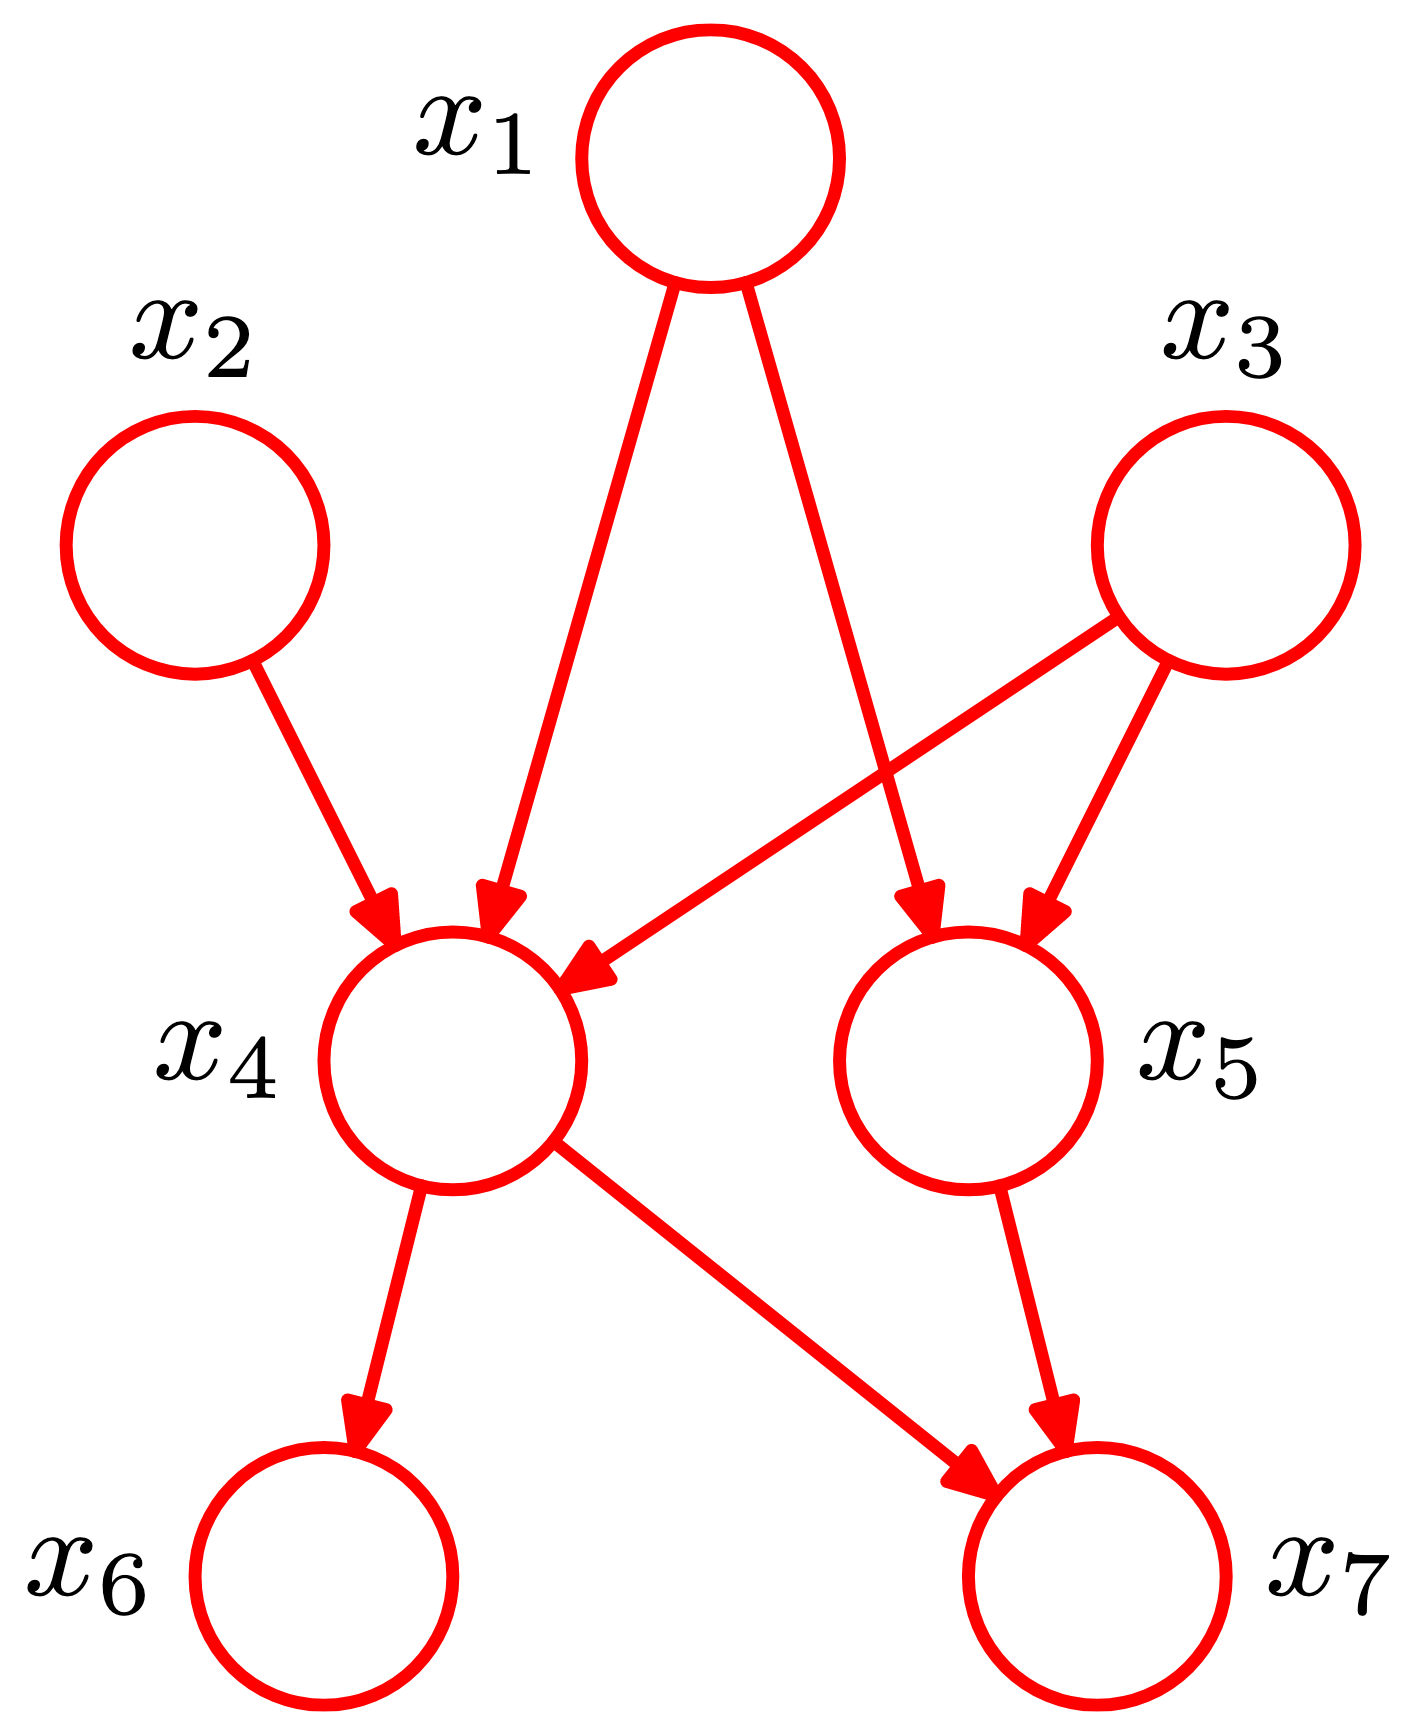
\includegraphics[scale=0.3]{BayesianNetwork1}
	\caption{Example of Bayes Network.}
	\label{fig:BayesianNetwork1}
\end{figure}
The $\mathcal{I}_\ell$ dependency is said to be local (${}_\ell$) since it's defined only wrt to a single variable. \newline
A part from the structure, we need also to have a probability distribution. Let's consider a dataset $\mathcal{D}$ in which all variables are tied with the other by a distribution $p$ which is a joint distribution. We'd like to represent qualitatively with a graph such distribution.\newline
Since the Bayesian Network depends on the independences, it's possible to create a set $\mathcal{I}(p)$ of these by looking at the distribution $p$.\newline
$\mathcal{G}$ is an \textit{independency map} (\textbf{I-map}) for $p$ if $p$ satisfies the local independencies in $\mathcal{G}$:
\[
	\mathcal{I}_\ell(\mathcal{G})\subseteq\mathcal{I}(p)
\]
The sufficient condition for $\mathcal{G}$ to be valid is that all the independences are also in $p$, while the opposite is not always true. Indeed, if some independence from $p$ cannot be modelled into $\mathcal{G}$ via qualitative definition, then they must be modelled quantitatively. \newline
Now we can describe $p$ in terms of the graphical model, that is we can \textbf{factorize} the distribution based on the structure of the model.
\begin{theorem}
$p$ is said to factorize according to $\mathcal{G}$ if:
\begin{equation}
	p(x_1,\hdots,x_m)=\Prod_{i=1}^mp(x_i\vert Parents_{x_i})
	\label{eq:BayesianNetworkFactorization}
\end{equation}
\label{theo:BayesianNetworkFactorization}
\end{theorem}
Mind that this is a double implication: if $\mathcal{G}$ is an I-map for $p$, then $p$ factorizes according to $\mathcal{G}$, then it's true also that if $p$ factorizes according to $\mathcal{G}$, then $\mathcal{G}$ is an I-map for $p$. 
This can be proven as follows.
\begin{proof}
\textit{I-map$\Rightarrow$ factorization}\newline 
If $\mathcal{G}$ is an I-map for $p$, then $p$ satisfies at least these local independences:
\[
\{\forall i~x_i\perp \ND_{x_i}\vert Parents_{x_i} \}
\]
It's possible to order the variable in a topological order relative to $\mathcal{G}$, i.e.:
\[
x_i\rightarrow x_j\Rightarrow i<j
\]
That is the parents have a lower id than the children. Let us now decompose the joint probability using the chain rule as:
\[
p(x_1,\hdots,x_m)=\Prod_{i=1}^mp(x_i\vert x_1,\hdots ,x_{i-1})
\]
Finally local independences imply that for each $x_i$:
\[
p(x_i\vert x_1,\hdots, x_{i-1})=p(x_i\vert Parents_{x_i})
\]
Which by substitution:
\[
p(x_1,\hdots,x_m)=\Prod_{i=1}^m p(x_i\vert Parents_{x_i})
\]
\end{proof}
\noindent Now we need to prove the inverse:
\begin{proof}
Factorization$\Rightarrow$ I-map\newline
If $p$ factorizes according to $\mathcal{G}$, the joint probability can be written as 
\[
p(x_1,\hdots,x_m)=\Prod_{i=1}^mp(x_i\vert Parents_{x_i})
\]
Said $\mathcal{X}$ the set of all variables $x_i$: $\mathcal{X}=\{x_1,\hdots,x_m\}$, let's consider variable $x_m$ (repeat the following steps for the other variable), it's possible to write by the product and sum rules:
\[
p(x_i\vert x_1,\hdots,x_{m-1})=\cfrac{p(x_1,\hdots,x_{m})}{p(x_1,\hdots,x_{m-1})}=\cfrac{p(x_1,\hdots,x_{m})}{\Sum_{x_m}p(x_1,\hdots,x_{m})}
\]
Applying factorisation and isolating the only term containing $x_m$ we get:
\[
	p(x_i\vert x_1,\hdots,x_{m-1})=\cfrac{\Prod_{i=1}^mp(x_i\vert Parents_{x_i})}{\Sum_{x_m}\Prod_{i=1}^mp(x_i\vert Parents_{x_i})}=
\]
\[
	=\cfrac{p(x_m\vert Parents_{x_m})\cancel{\Prod_{i=1}^{m-1}p(x_i\vert Parents_{x_i})}}{\cancel{\Prod_{i=1}^{m-1}p(x_i\vert Parents_{x_i})} \cancel{\Sum_{x_m}p(x_m\vert Parents_{x_m})}}
\]
The sum cancels out because summing all the value of a variable equals to 1. \newline
Hence:
\[
	p(x_i\vert x_1,\hdots,x_{m-1})=p(x_m\vert Parents_{x_m})
\]
\end{proof}
\noindent For example consider Figure~\ref{fig:BayesianNetwork1}. It's possible to write:
\[
	p(x_1,\hdots x_7)=p(x_1)p(x_2)p(x_3)p(x_4\vert x_1,x_2,x_3)p(x_5\vert x_2,x_3)p(x_6\vert x_4)p(x_7\vert x_4,x_5)
\]
Mind that the joint probability $p(x_1, \hdots, x_7)$ is largely influenced by the probability of node 4: $p(x_4\vert x_1, x_2, x_3)$. Now let's suppose that each variable defined a simple binary value, then the total number of possibility would be $2^7$, against the $2^4$ we found right now. This allows to be able to work with a lot of variables. \newline
\begin{definition}[Bayesian Network]
A Bayesian Network is a pair $(\mathcal{G}, p)$ where $p$ factorizes over $\mathcal{G}$ and its represents as a set of conditional probability distribution associated with the nodes of $\mathcal{G}$
\end{definition}
%
%
\subsection{Example}%TODO non so a cosa serva questo esempio
Let's consider another example: genes A and B have independent prior probabilities and gene C can be enhanced by both A and B, with the following probability tables:
\begin{center}
	\begin{tabular}{c|c|cp{2cm}c|c|c}
		Gene&Value&$P(value)$&&Gene&Value&$P(value)$\\
		\cline{1-3}\cline{5-7}
		A&Active&0.3&&B&Active&0.3\\
		A&Inactive&0.7&&B&Inactive&0.7\\
	\end{tabular}
\end{center}
\begin{table}[!h]
	\centering
	\begin{tabular}{cc|cc|cc}
		\mc{2}{c|}{}&\mc{4}{c}{A}\\
		\mc{2}{c|}{}&\mc{2}{c}{Active}&\mc{2}{c}{Inactive}\\
		\hline
		\mc{2}{c|}{}&\mc{2}{c|}{B}&\mc{2}{c}{B}\\
		\mc{2}{c|}{}&Active&Inactive&Active&Inactive\\
		\hline
		C&Active&0.9&0.6&0.7&0.1\\
		C&Inactive&0.1&0.4&0.3&0.9
	\end{tabular}
	\caption{Table showing $p(A,B,\vert C)$.}
\end{table}
%
%
\subsection{Conditional Independence}
First of let's recall Definition~\ref{def:Independence}: two variables $a,b$ are said to be independent written $a\perp b\vert\emptyset$ if: 
\[
p(a,b)=p(a)p(b)
\]
\begin{definition}[Conditional Independence]
Two variables $a,b$ are conditionally independent given $c$, written $a\perp b\vert c$ if:
\[
p(a,b\vert c)=p(a\vert c)p(b\vert c)
\]
\end{definition}
Graphical models allow to directly verify them through the \textbf{d-separation} criterion.
%
%
%
\section{D-separation}
Looking at some simpler graphs, some dependency rules can be inferred and then used on larger graphs by applying them to subgraphs.
%
%
\subsection{Two Nodes}
Given two nodes, or they are independent, hence they are not connected, or they are dependent, hence they are connected.
%
%
\subsection{Three Nodes}
%
\subsubsection{Tail-To-Tail}
Also known as \textit{common cause}.
\begin{center}
	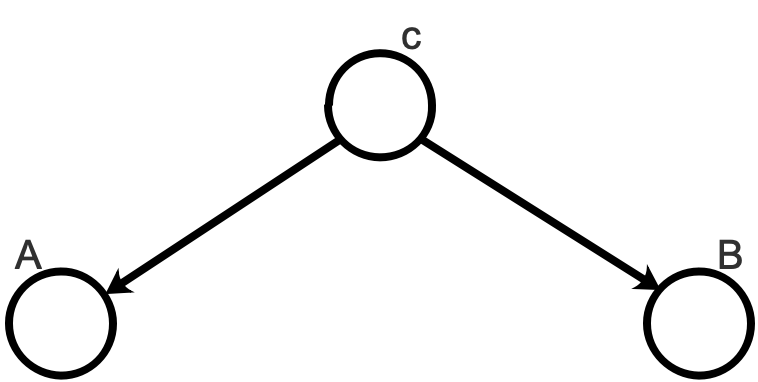
\includegraphics[width=0.4\linewidth]{tailToTailNoGiven}
\end{center}
As for the factorization Equation~\ref{eq:BayesianNetworkFactorization}, the joint distribution can be expressed as:
\[
	p(a,b,c)=p(a\vert c)p(b\vert c)p(c)
\]
The tail-to-tail case says that $a$ and $b$ are \textit{not independent}, written $a \not\!\perp\!\!\!\perp b$. %$a\downmodels b\vert\emptyset$
If $c$ is not given then we have that:
\[
	p(a,b)=\Sum_cp(a\vert c)p(b\vert c)p(c)\neq p(a)p(b)
\] 
On the contrary, if $c$ is given, then they are \textit{conditionally independent}:
\[
p(a,b\vert c)=\cfrac{p(a,b,c)}{p(c)}=p(a\vert c)p(b\vert c)
\] 
\begin{center}
	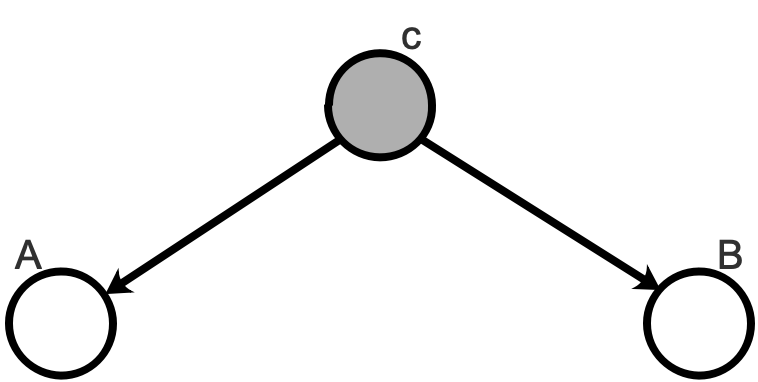
\includegraphics[width=0.4\linewidth]{tailToTailGiven}
\end{center}
Let's consider an example: a company needs to choose the most intelligent ($I$) student between more students. For each student the variables grade $(G)$ and score ($S$) are given. The following graph can be drawn since if the student is intelligent, then it should be seen in both grades and scores. \newline
\begin{minipage}[htp]{\linewidth}
	\begin{minipage}[t]{0.48\linewidth}
		\begin{center}
			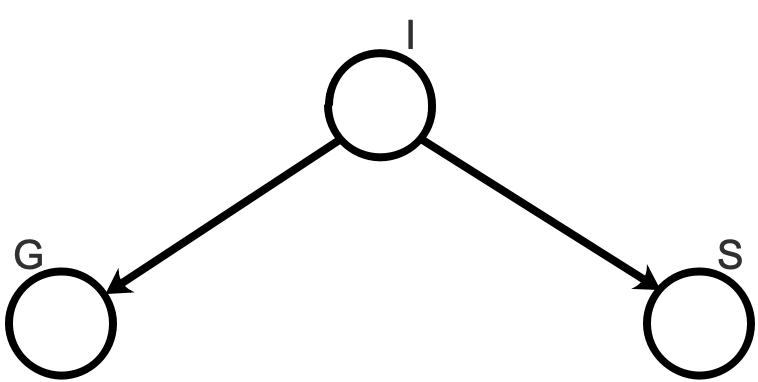
\includegraphics[width=0.7\linewidth]{tailToTailExample1}
		\end{center}
		$G$ and $S$ are directly correlated, for example observing high scores could be indication of having a higher intelligence and hence also higher grades. 
	\end{minipage}
	\hspace{0.04\linewidth}
	\begin{minipage}[t]{0.48\linewidth}
		\begin{center}
			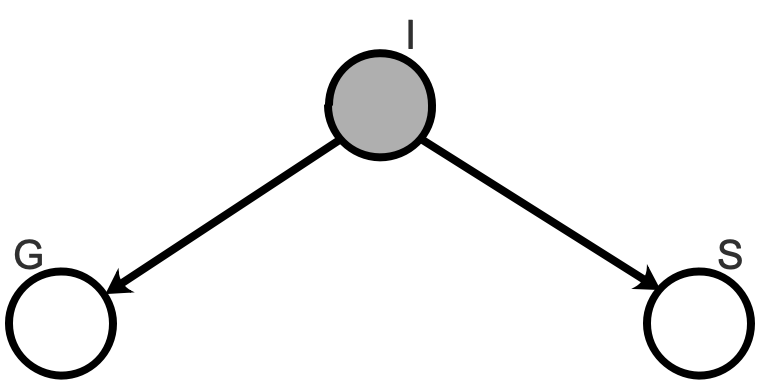
\includegraphics[width=0.7\linewidth]{tailToTailExample2}
		\end{center}
		$G$ and $S$ are not directly dependent since once intelligence has been observed, the correlation disappear and nor $G$ gives more information $S$, nor $S$ gives more information about $G$ than the what we already know. 
	\end{minipage}
\end{minipage}
%
\subsubsection{Head-To-Tail}
Also known as \textit{indirect causal effect}.
\begin{center}
	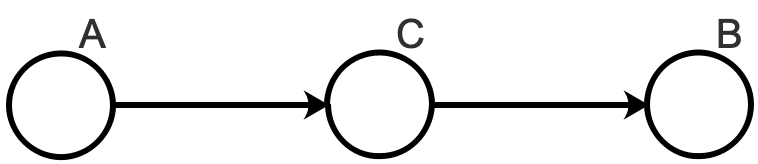
\includegraphics[width=0.4\linewidth]{HeadToTailNoGiven}
\end{center}
The joint distribution can be expressed as:
\[
p(a,b,c)=p(b\vert c)p(c\vert a)p(a)=p(b\vert c)p(a\vert c)p(c)
\]
If $c$ is not given, then then $a$ and $b$ are \textit{not independent}:
\[
p(a,b)=p(a)\Sum_cp(b\vert c)p(c\vert a)\neq p(a)p(b)
\]
If instead $c$ is given, then $a$ and $b$ are conditionally independent:
\[
p(a,b\vert c)=\cfrac{p(b\vert c)p(a\vert c)p(c)}{p(c)}=p(b\vert c)p(a\vert c)
\]
\begin{center}
  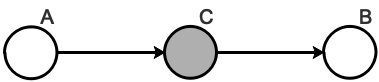
\includegraphics[width=0.4\linewidth]{HeadToTailGiven}
\end{center}
As before, let's consider the example of the intelligence of a student. \newline
\begin{minipage}[htp]{\linewidth}
	\begin{minipage}[t]{0.48\linewidth}
		\begin{center}
			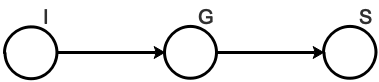
\includegraphics[width=0.7\linewidth]{HeadToTailExample1}
		\end{center}
    Intuitivly, if we observe that the student is intelligent, then we are more inclined to believe that it's grades $G$ are good and that they will have a better score at the interview $S$, that is the probability of these latter events is higher conditioned on the observation that the student is intelligent. 	
	\end{minipage}
	\hspace{0.04\linewidth}
	\begin{minipage}[t]{0.48\linewidth}
		\begin{center}
			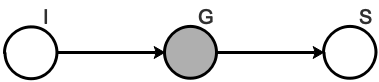
\includegraphics[width=0.7\linewidth]{HeadToTailExample2}
		\end{center}
    Instead if we assume that $G$ is observed, then it's intelligence no longer influences the score of the interview.
	\end{minipage}
\end{minipage}
%
\subsubsection{Head-To-Head}
Also known as \textit{common effect}.
\begin{center}
	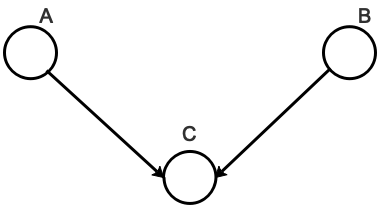
\includegraphics[width=0.4\linewidth]{HeadToHeadNoGiven}  
\end{center}
The joint distribution can be expressed as:
\[
  p(a,b,c)=p(c\vert a, b)p(a)p(b)
\]
If $c$ is not given, then then $a$ and $b$ are \textit{independent}:
\[
  p(a,b)=\Sum_cp(c\vert a, b)p(a)p(b)=p(a)p(b)
\]
If instead $c$ is given, then $a$ and $b$ are not conditionally independent, hence they are conditionally dependent:
\[
p(a,b\vert c)=\cfrac{p(c\vert a,b)p(a)p(b)}{p(c)}\neq p(a\vert c)p(b\vert c)
\]
\begin{center}
  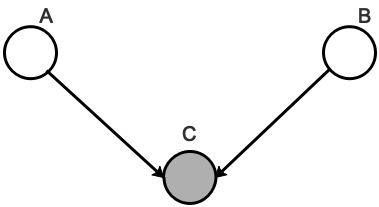
\includegraphics[width=0.4\linewidth]{HeadToHeadGiven}
\end{center}
Let's consider one last time the example of the student that is to be hired from a company. We have said that if $c$ is not given, then $a$ and $b$ are independent, while if $c$ is given they are dependent. Indeed, if $c$ was the score of a test, then the student ($G$) and it was low, we could think that they are actually not that smart, but then if we were to observe that the test was difficult, then we could think that actually they are not \textit{not} intelligent. Hence, $a$ and $b$ are actually correlated if $c$ is given. 
\begin{center}
  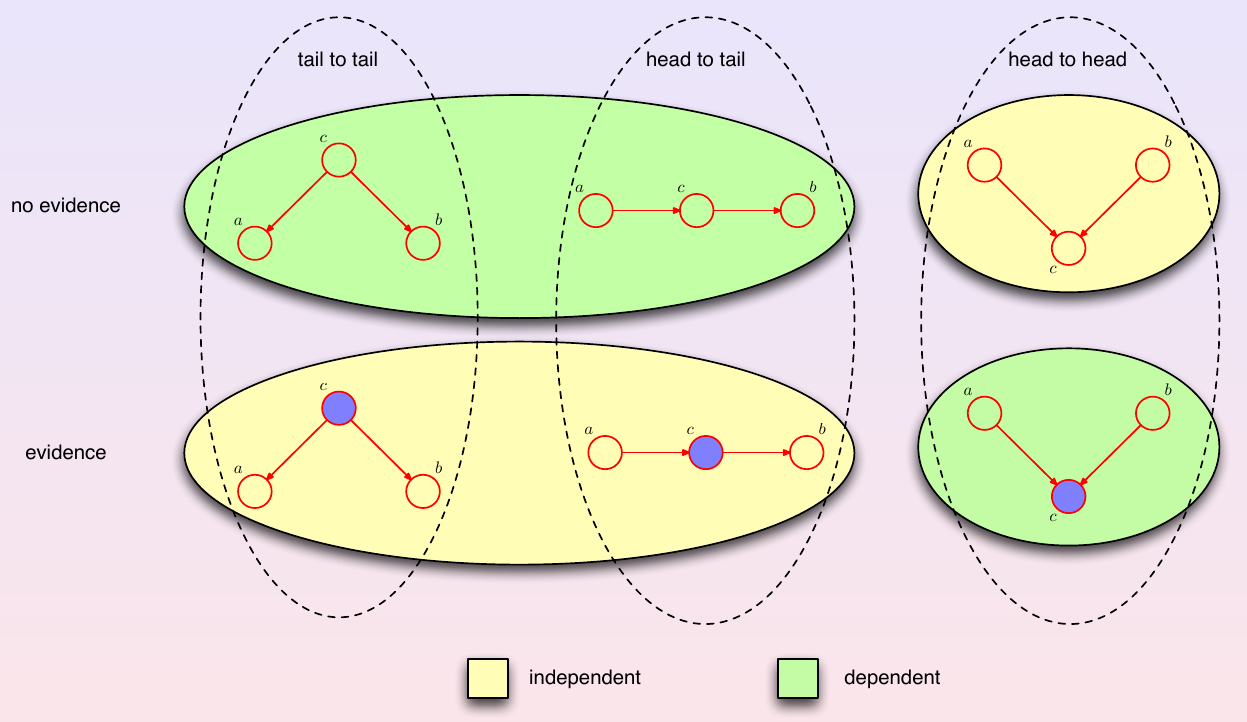
\includegraphics[width=0.8\linewidth]{DSeparationRecap}
\end{center}
\myparagraph{Example Head-To-Head Example}
Let's consider a fuel system of a car. The fuel system is make of:
\begin{itemize}
  \item Battery $B$: can either be charged ($B=1$) or flat ($B=0$);
  \item Fuel tank $F$: can either be full ($F=1$) or empy ($F=0$);
  \item Electric fuel gauge $G$: either full ($G=1$) or empty ($G=0$).
\end{itemize}
Let's now say that the probability of the battery to be charged is $P(B=1)=0.9$ and the probability for the fuel tank to be full is $P(F=1)=0.9$. \newline
The electric fuel gauge is conditioned on both:
\begin{center}
  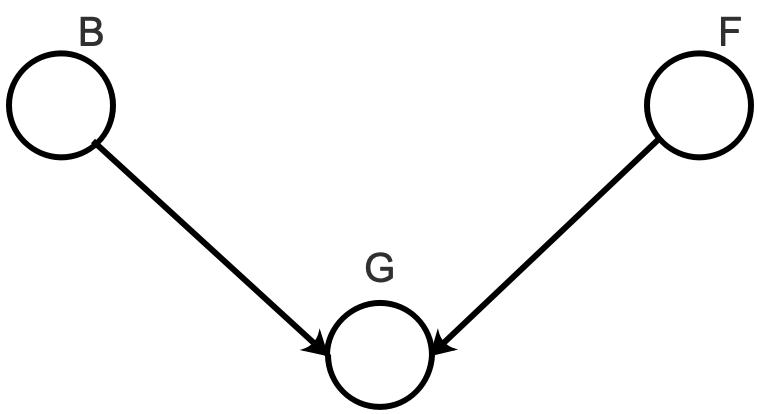
\includegraphics[width=0.5\linewidth]{FuelTankExample1NoGiven}
\end{center}
\[
  \begin{array}{ll}
    P(G=1\vert B=1,F=1)=0.8&P(G=1\vert B=1,F=0)=0.2\\
    P(G=1\vert B=0,F=1)=0.2&P(G=1\vert B=0,F=0)=0.1\\
  \end{array}
\]
We want to compute the probability of having an empty tank:
\[P(F=0)=1-P(F=1)=0.1\]
What would happen to the probability if we were to notice that the fuel gauge was empty? In particular let's compute the probability of the fuel tank to be empty given the fact that the fuel gauge is empty $P(F=0\vert G=0)$. Such probability is not given, hence we need to find it. To compute $P(F=0\vert G=0)$ we could use Bayes:
\[P(F=0\vert G=0)=\dfrac{P(G=0\vert F=0)P(F=0)}{P(G=0)}\]
We need to compute $P(G=0\vert F=0)$ and $P(G=0)$ but they are easier to compute by the product rule:
\[
\begin{array}{ll}
  P(G=0\vert F=0)&=\Sum_{B\in\{0,1\}}P(G=0,B\vert F=0)\\
                 &=\Sum_{B\in\{0,1\}}P(G=0\vert B,F=0)P(B\vert F=0)\\
                 &=\Sum_{B\in\{0,1\}}P(G=0\vert B,F=0)P(B)\\
                 &=P(G=0\vert B=0, F=0)P(B=0)+P(G=0\vert B=1, F=0)P(B=1)\\
                 &=0.9\cdot0.1+0.8\cdot 0.9=0.81
\end{array}
\]
Notice that the passage from the second to the third equation it's possible since $B$ and $F$ are independent, hence $P(B\vert F=0)=P(B)$.\newline 
Similarly $P(G=0)$ is given by:
\[
\begin{array}{ll}
  P(G=0)&=\Sum_{B\in\{0,1\}}\Sum_{F\in\{0,1\}}P(G=0,B,F)\\
        &=\Sum_{B\in\{0,1\}}\Sum_{F\in\{0,1\}}P(G=0\vert B,F)P(B)P(F)=0.315  
\end{array}
\]
In the end it's possible to see that by observing the fact that the fuel gauge is empty, then the probability of the fuel tank of being actually empty increases:
\[P(F=0\vert G=0)=\dfrac{P(G=0\vert F=0)P(F=0)}{P(G=0)}\simeq 0.257\]
Not as much as one would expect, but this is due to strong prior and an unreliable gauge. \newline
Now let's consider the case in which we knew that also the battery is flat. How does the probability $P(F=0\vert G=0,B=0)$ change knowing this information? \newline
It's possible to apply again Bayes Theorem and have:
\[P(F=0\vert G=0, B=0)=\dfrac{P(G=0\vert F=0,B=0)P(F=0\vert B=0)}{P(G=0\vert B=0)}\]
\begin{definition}[Active Trail]
  Let's consider a graph with three node $X,Y,Z$ connected as in one of the cases before. The trail $X\rightleftharpoons Y\rightleftharpoons Z$ is said to be \textit{active} if information can flow from $X$ to $Y$ via $Z$.
  \begin{itemize}
    \item Head-to-Tail $X\rightarrow Z\rightarrow Y$ is active if and only if $Z$ \textbf{is not} observed;
    \item Tail-to-Tail $X\leftarrow Z\rightarrow Y$ is active if and only if $Z$ \textbf{is not} observed;
    \item Head-to-Head $X\rightarrow Z\leftarrow Y$ is active if and only if $Z$ \textbf{is} observed;
  \end{itemize}
\end{definition}
%
%
\subsection{d-Separation -- General Case}
Obviously the majority of the graphs is not made of three nodes, but has many nodes. Suppose that we want to find a path that allows to go from one group nodes holding evidence to another. We can say whether this is possible or not by applying the before rules and by adding the following rule: a head-to-head node $c$ unblocks the dependency path between its parents if either itself or \textit{any of its descendants} receives evidence. \newline
\begin{definition}[Descendant]
  A descendant of a node $x$ is any node which can be reached from $x$ with a path following the direction of the arrows.   
\end{definition}
\begin{theorem}[$d$-Separation General Case]
  Let $\mathcal{G}$ be a Bayesian Network structure and $X_1\rightleftharpoons\hdots\rightleftharpoons X_n$ a trail in $\mathcal{G}$. Let $\vect{Z}$ be a subset of observed variables. The trail $X_1\rightleftharpoons\hdots\rightleftharpoons X_n$ is active given $\vect{Z}$ if:
  \begin{itemize}
    \item Whenever we have a head-to-head structure $X_{i-1}\rightarrow X_i\leftarrow X_{i+1}$, then $X_i$ or one of its descendants are in $\vect{Z}$;
    \item No other node along the trail is in $\vect{Z}$.
  \end{itemize}
\end{theorem}
Note that if $X_1$ or $X_n$ are in $\vect{Z}$, then the trail is not active. \newline
\begin{definition}[Path Blocked]
  A path is said to be blocked if it includes at least one node such that either:
  \begin{itemize}
    \item The arrows on the path meet tail-to-tail or head-to-tail at the node and it is in $C$, or
    \item The arrows on the path meet head-to-head at the node and neither it nor any of its descendants is in $C$. 
  \end{itemize}
\end{definition}
\begin{definition}[General d-separation Criterion]
  Given a generic Bayesian Network and nonintersecting arbitrary sets of nodes $A,B,C$, the sets $A$ and $B$ are d-separated by $C$, written $\dsep{A;B\vert C}$ if all paths from any node in $A$ to any node in $B$ are blocked.
  \label{def:dSeparation}
\end{definition}
Note that d-separation \textit{implies conditional independence}: the sets $A$ and $B$ are independent given $C$, written $A\perp B\vert C$ if they are d-separated by $C$.
%
\subsubsection{Example 1}
Let's consider the following graph:
\begin{center}
  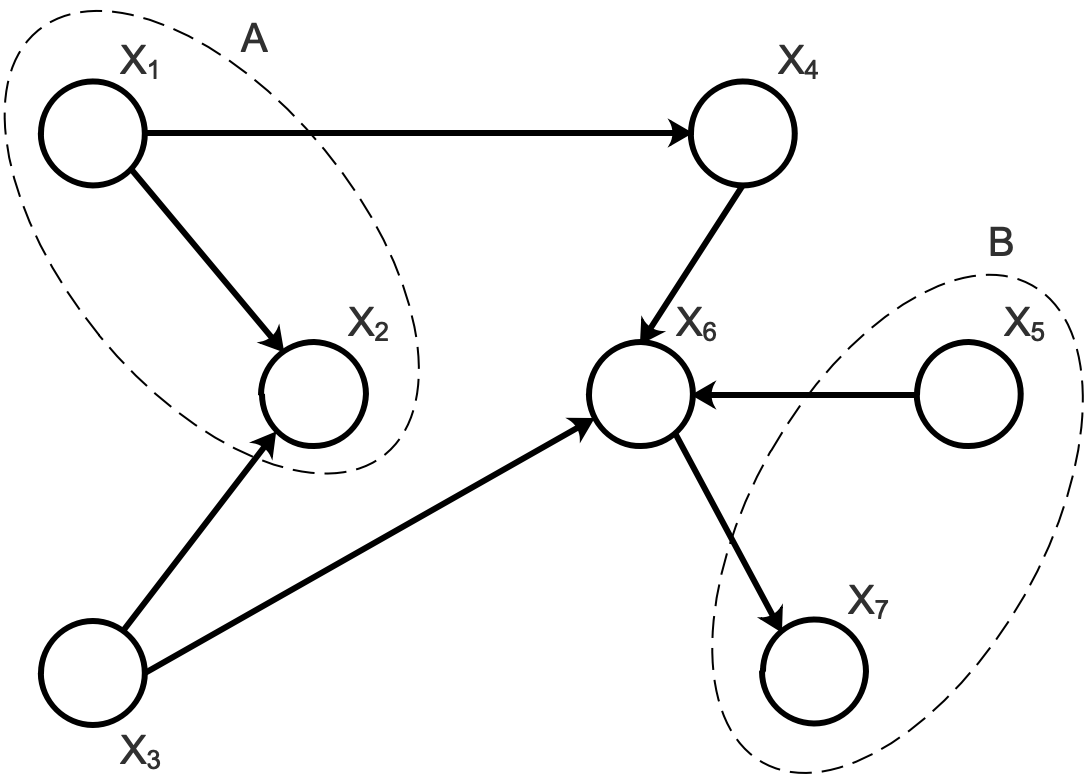
\includegraphics[width=0.7\linewidth]{dSeparationExample1_1}
\end{center}
and three independent sets: $A=\{X_1,X_2\}, B=\{X_5,X_7\}, C=\emptyset$. By applying the rules we need to find a possible path from one set to another. For example let's consider a first possibility made of the path $X_1\rightarrow X_4\rightarrow X_6\leftarrow x_5$: the first three nodes are in a head-to-tail structure, we do not have any information regarding $X_4$, hence the path is active till this point. $X_4\rightarrow X_6\leftarrow X_5$ is a head-to-head structure and there is no evidence on $X_6$, hence the path is blocked. \newline
Let's instead consider the path: $X_1\rightarrow X_4\rightarrow X_6\rightarrow X_7$. We saw that the first three nodes are in a head-to-tail structure and there is no evidence, so the trail is active. Let's then look at the last three nodes: $X_4\rightarrow X_6\rightarrow X_7$: this is head-to-tail structure and there is no evidence on $X_6$, hence the trail is active and an actual path from the set $A$ to the set $B$ could be found. \newline
It's possible to find also a path starting from $X_2$: $X_2\leftarrow X_3\rightarrow X_6 \rightarrow X_7$ which actually works because the first three nodes are in a tail-to-tail structure and there is no evidence on $X_3$, hence the trail is active, and the last three nodes are in a head-to-tail structure with no evidence on $X_6$. \newline
Similarly to before, the path $X_2\leftarrow X_3\rightarrow X_6\rightarrow X_5$ does not work because the last three nodes are in a head-to-head structure and there is no evidence on $X_6$.
%
\subsubsection{Example 2}
Let's consider the case in which $X_6$ is given evidence:
\begin{center}
  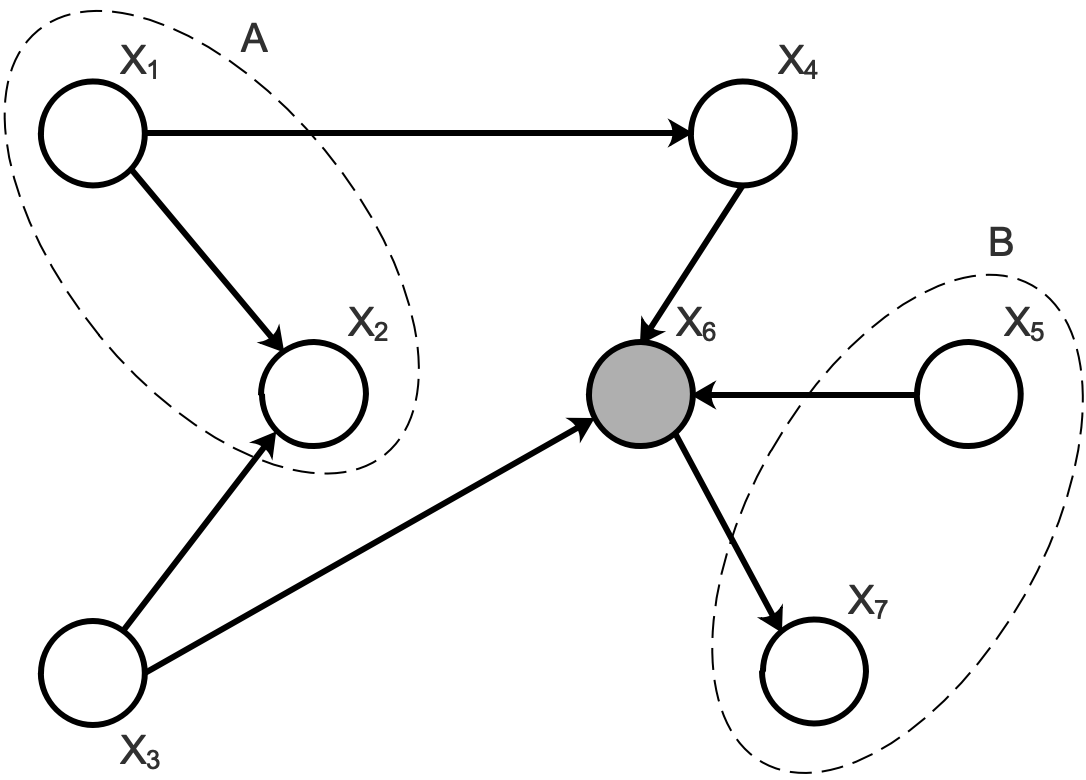
\includegraphics[width=0.7\linewidth]{dSeparationExample1_2}
\end{center}
In this case the path $X_1\rightarrow X_4\rightarrow X_6 \leftarrow X_5$ is a correct path since $X_4$ holds no evidence hence the trail $X_1\rightarrow X_4\rightarrow X_6$ is active and $X_6$ holds evidence, so the structure $X_4\rightarrow X_6\leftarrow X_5$ is active too. 
%
\subsubsection{Example 3}
Let's consider the following cases and decide whether $a$ and $b$ are d-separated:
\begin{center}
  \begin{minipage}[t]{\linewidth}
    \begin{minipage}[t]{0.48\linewidth}
      \begin{center}
        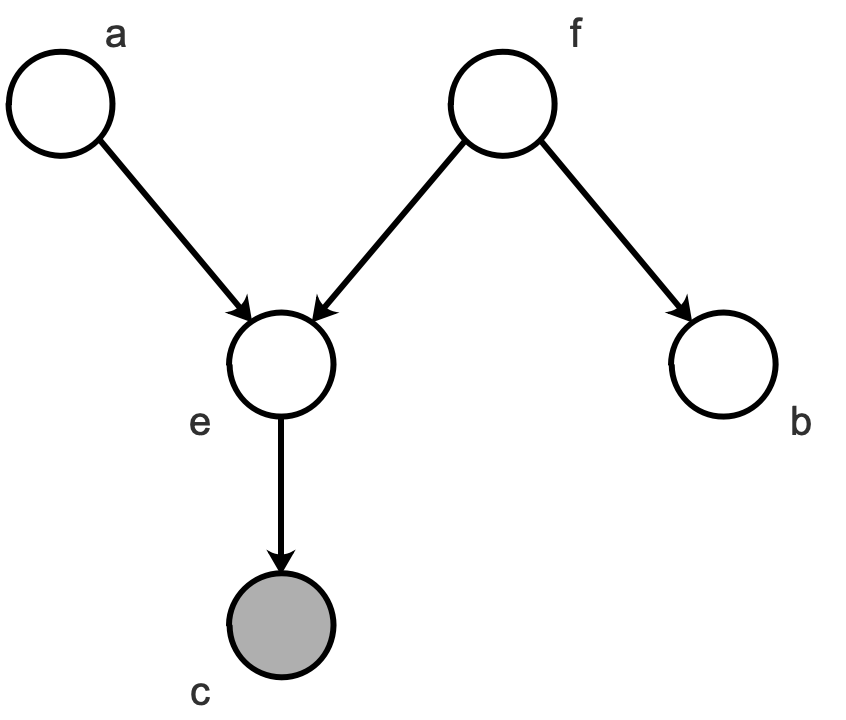
\includegraphics[width=0.8\linewidth]{dSeparationExample2_1}
      \end{center}
      In this case, the first three nodes meet a head-to-head structure and we have that $c$, which is a descendant of $e$, has evidence, hence the trail is active. The last three nodes are in a tail-to-tail structure, $f$ does not have any evidence, hence the path is valid and $a$ and $b$ are not d-separated since there exists a path from $a$ to $b$. 
    \end{minipage}
    \hspace{0.03\linewidth}
    \begin{minipage}[t]{0.48\linewidth}
      \begin{center}
        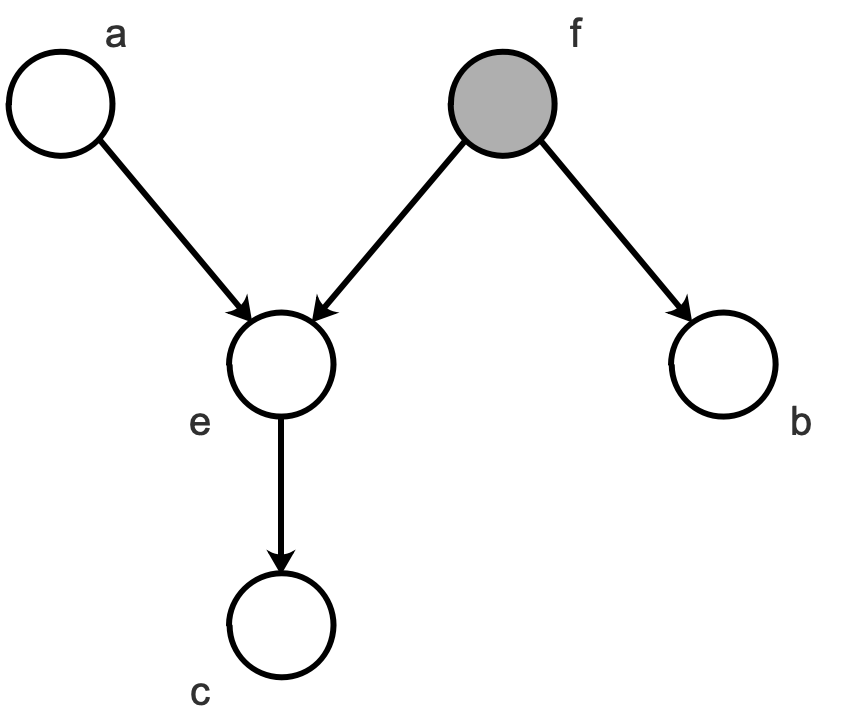
\includegraphics[width=0.8\linewidth]{dSeparationExample2_2}
      \end{center}
      It's immediate to see that $f$ is observed, hence the trail $e\leftarrow f\rightarrow b$ is not active, and also there is no evidence for $e$ or any of its descendants. By Definition~\ref{def:dSeparation}, $a$ and $b$ are d-separated given $f$: $a\perp b\vert f$.
    \end{minipage}
  \end{minipage}
\end{center}
%
%
%
\section{Bayesian Networks independences}
We saw how local independences work, that is independences between nodes, now we are going to define also global dependencies. \newline
\begin{definition}[Local Independece]
  A Bayesian Networks structure $\mathcal{G}$ encodes a set of local independence assumptions:
  \[\mathcal{I}_l(\mathcal{G})=\{\forall i~ x_i\perp \text{nondescendants}_{x_i}\vert \text{parents}_{x_i}\}\]
\end{definition}
\begin{definition}[Global Independence]
  A Bayesian Network structure $\mathcal{G}$ encodes a set of global (Markov) independence assumptions:
  \[\mathcal{I}(\mathcal{G})=\{(A\perp B\vert C):\dsep{A;B\vert C}\}\]
\end{definition}
Notice that the global independences contain the local independences.
%
%
%
\section{$l$-Equivalence}
We can notice that different structures actually encode the same set of independences assumptions. Let's consider for example head-to-head in one direction or in the other: if the intermediate node does not present evidence, then the two structures encode the same independence. In Figure~\ref{fig:lEquivalence} are shown two equivalence classes. 
\begin{figure}[htp]
  \centering
  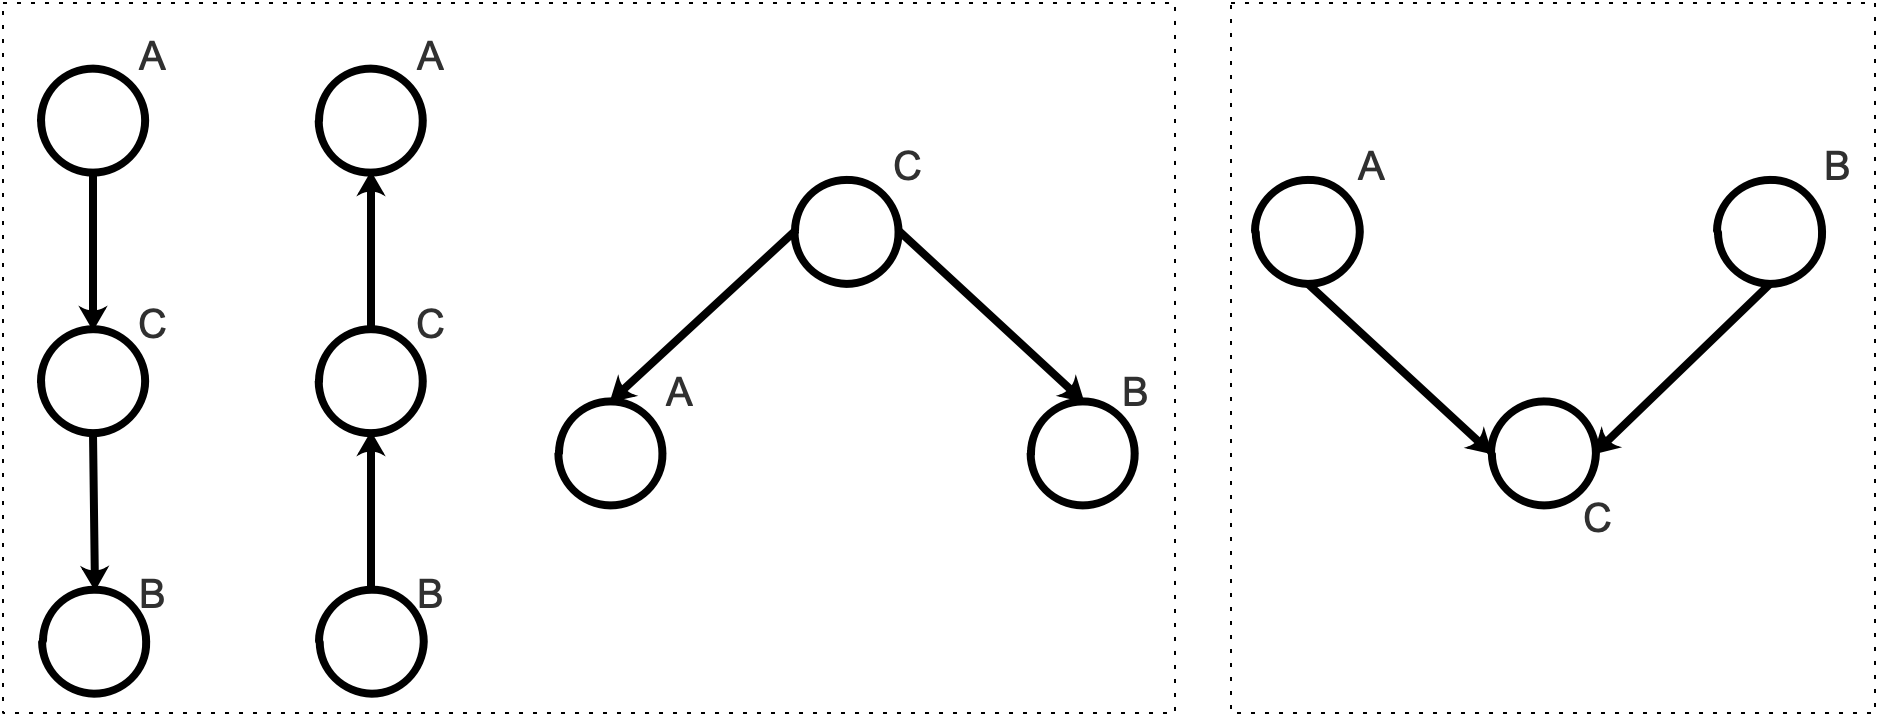
\includegraphics[width=0.8\linewidth]{lEquivalence}
  \caption{Two equivalence classes.}
  \label{fig:lEquivalence}
\end{figure}
\begin{definition}[$l$-Equivalence]
  Two Bayesian Networks structures $\mathcal{G}$ and $\mathcal{G}'$ are $l$ equivalent if $\mathcal{I}(\mathcal{G})=\mathcal{I}(\mathcal{G}')$.
\end{definition}
The space of Bayesian Network structures over the set of nodes $\mathcal{X}$ is partitioned into a set of mutually exclusive and exhaustive $l$-equivalence classes. \newline
Note that $l$-equivalence of two graphs implies that any distribution $P$ that can be factorized over on of these graphs can be factorized over the other too. Furthermore, there is no intrinsic property $P$ that would allow us to associate it with one graph rather than an equivalent one. In other words, although we can determine, for a distribution $P(X,Y)$, whether $X$ and $Y$ are correlated, there is nothing in the distribution that can help us determine whether the correct structure is $X\rightarrow Y$ or $Y\rightarrow X$. \newline
\begin{definition}[Skeleton]
  The skeleton of a Bayesian network graph $\mathcal{G}$ over a set of nodes $\mathcal{X}$ is an undirected graph over $\mathcal{X}$ that contains an edge $\{X,Y\}$ for every edge $(X,Y)$ in $\mathcal{G}$.
\end{definition}
It's possible to prove that if two structures $\mathcal{G}$ and $\mathcal{G}'$ have the same skeleton and the same set of v-structures, then they are $l$-equivalent. 
\begin{center}
  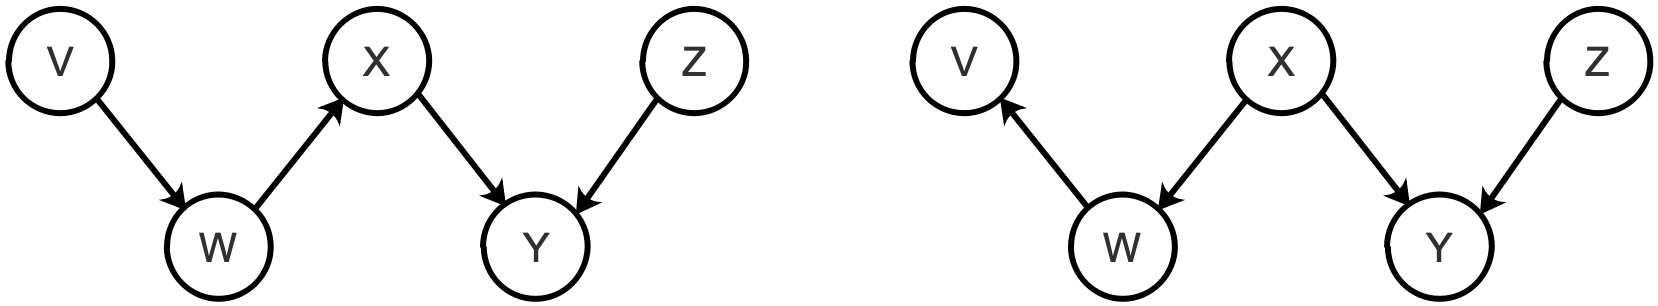
\includegraphics[width=0.7\linewidth]{lEquivalenceSkeleton}
\end{center}
Considering the above structures, they are $l$-equivalent since they have the same skeleton and the same v-structure ($X\rightarrow Y\leftarrow Z$). \newline
This is actually a \textit{sufficient condition}. Instead it's possible to have a \textit{necessary and sufficient condition} by considering also \textbf{immoralities}.
\begin{definition}[Immorality]
  A v-structure $X\rightarrow Z\leftarrow Y$ is an immorality if there is no direct edge between $X$ and $Y$. If there is such an edge, it is called a \textbf{covering edge} for the v-structure.  
\end{definition}
\begin{center}
  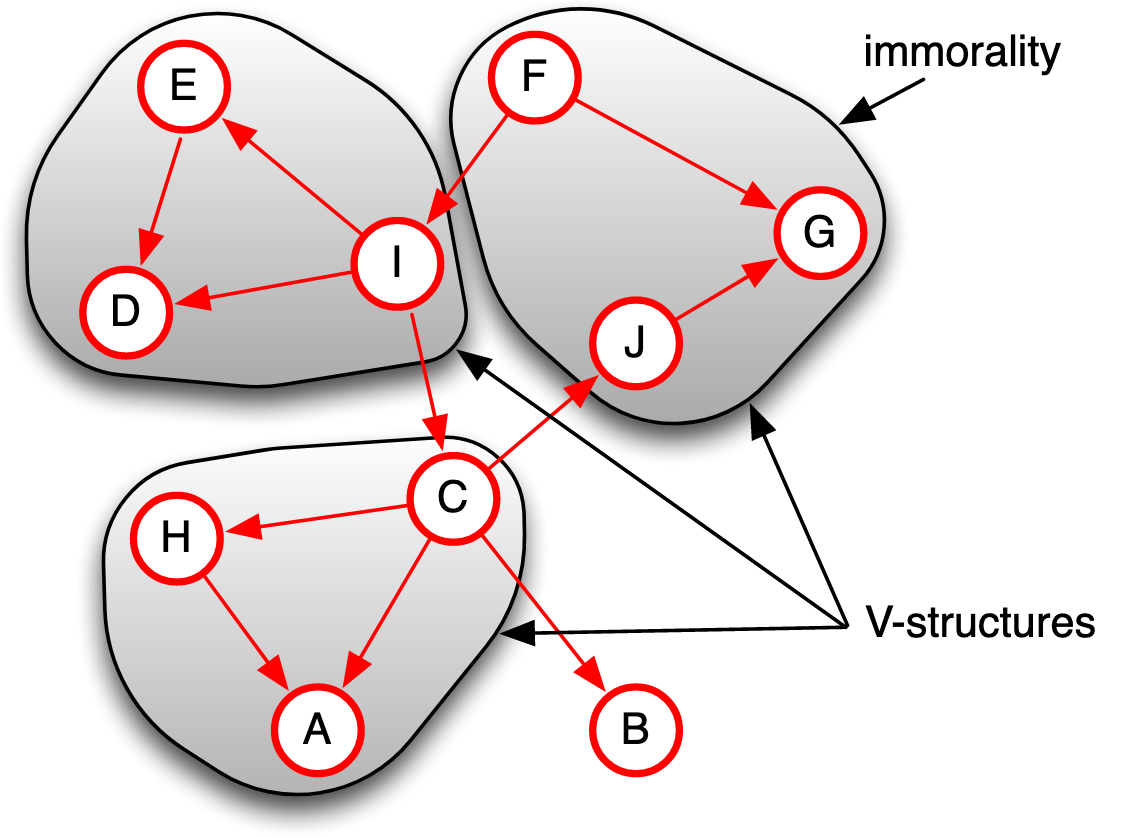
\includegraphics[width=0.6\linewidth]{lEquivalenceImmorality}
\end{center}
It's possible to notice that the v-structure $F\rightarrow G\leftarrow J$ is different from the other two since there is no edge between $F$ and $J$. This implies that such v-structure is an immorality, while the others are not immoralities. \newline
The following necessary and sufficient condition can be expressed an proven:
\begin{theorem}
  Let $\mathcal{G}_1$ and $\mathcal{G}_2$ be two graphs over a set of nodes $\mathcal{X}$. Then $\mathcal{G}_1$ and $\mathcal{G}_2$ have the same skeleton and the same set of immoralities if and only if they are $l$-equivalent. 
\end{theorem}
%
%
\subsection{$l$-Maps}
There can be two types of of maps: \textit{minimal l-maps} and \textit{P-maps}, that is perfect maps. \newline
Notice that for a structure $\mathcal{G}$ to be an $l$-map for a distribution $p$, it does not need to encode all its independences, e.g., a fully connected graph is an $l$-map of any $p$ defined over its variables.
\begin{definition}[Minimal $l$-Map]
  A minimal $l$-map for a distribution $p$ is an $l$-map $\mathcal{G}$ which can't be reduced into a $\mathcal{G}'\subset \mathcal{G}$ that is also an $l$-map for $p$.
\end{definition}
To reduce an $l$-map to another $l$-map means that by removing some edges we obtain again a valid $l$-map. \newline
Note that by this definition, a minimal $l$-map for $p$ does not necessarily capture all the independences in $p$. On the contrary a perfect $P$-map does:
\begin{definition}[$P$-Map]
  A structure $\mathcal{G}$ is a perfect map $P$-map for a distribution $p$ if it captures all (and only) its independences:
  \[\mathcal{I}(\mathcal{G})=\mathcal{I}(p)\]
\end{definition}
Notice that a $P$-map is also a minimal $l$-map, while the opposite is not valid. \newline
There exists an algorithm that allows one to find a $P$-map for a distribution $p$, but it's exponential w.r.t. the \textit{in-degree} of the $P$-map, that is the maximum number of connections of the nodes. Moreover the algorithms returns an equivalence class rather than a single structure. \newline
Moreover there are some distributions for which is not possible to find $P$-maps. In these cases, indirect graphs called Markov Networks are used.
%
%
%
\section{Making Bayesian Networks}
The first step is to find a field-expert who can tell us the variables that we may need. For example, if we are trying to develop an algorithm to predict a disease, we need to know all the possible symptoms. \newline
The next step is to actually define the variables that can be observed or that you can be interested in predicting, also latent variables can be useful. \newline
By following \textit{causality} considerations, we try to add edges to the variables. This would allow us to have a more interpretable network and also a sparser one. \newline
Lastly we start to add the probabilities for the configurations and its best to (almost) never assign zero probabilities. If any data are available, we should use them to help in learning parameters, and also the structure. 
%
%
%
\section{Inference in Graphical Models}
Bayesian Networks, as all the graphical models, actually models a joint probability. \newline
Assume we have evidence $\vect{e}$ on the state of a subset of variables $\vect{E}$ in the model. Inference amounts at computing the posterior probability of a subset $\vect{X}$ of the non-observed variables given the observations:
\[P(\vect{X}\vert\vect{E}=\vect{e})=\dfrac{P(\vect{X}, \vect{E})}{P(\vect{E}=\vect{e})}\]
The problem consists in estimating such joint probabilities when dealing with a large number of variables: directly working on the full joint probabilities would require time exponential in the number o variables. For instance, if all $N$ variables are discrete and take one of $K$ possible values, a joint probability table has $K^N$ entries. 
\[P(\vect{X}\vert\vect{E}=\vect{e})=\dfrac{P(\vect{X}, \vect{E})}{P(\vect{E}=\vect{e})}=\Sum_{Y_1,\hdots,Y_n}P(\vect{X},Y_1,\hdots,Y_n,\vect{E}=\vect{e})\]
Our goal is to exploit the structure in graphical models to do inference more efficiently.
%
%
\subsection{Inference -- Chain}
The most simple structure we have seen is a chain of nodes where each variable has a connection to the following one. 
\begin{center}
  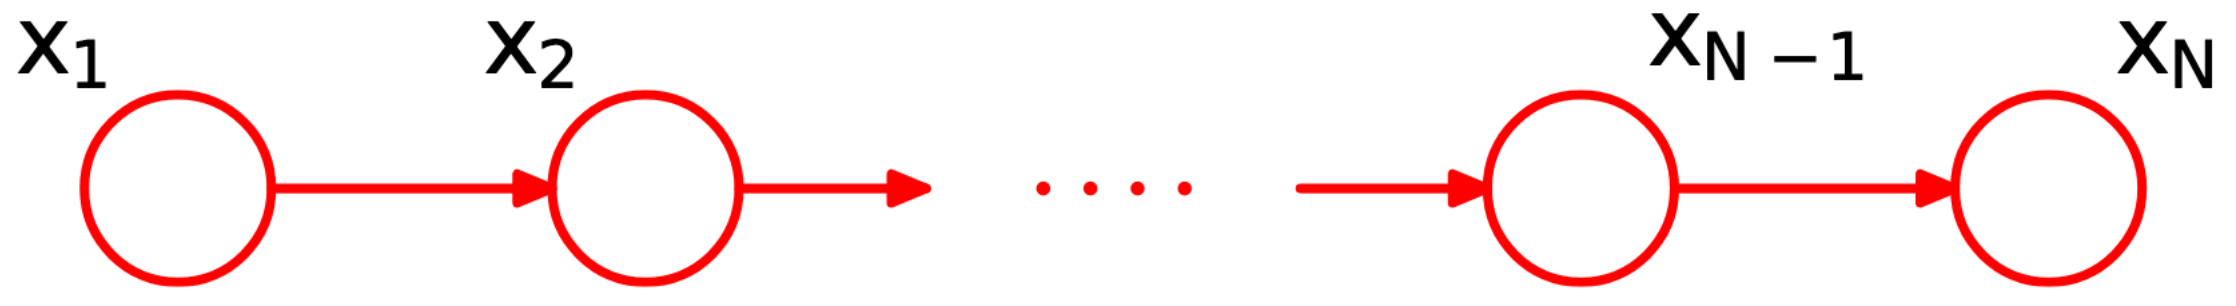
\includegraphics[width=0.7\linewidth]{InferenceChain}
\end{center}
In this way the probability of all variables in the chain becomes:
\[P(X)=P(X_1)\cdot P(X_2\vert X_1)\cdot \hdots \cdot P(X_{N}\vert X_{N-1})\]
The marginal probability of an arbitrary variable $X_i$ is:
\[P(X_i)=\Sum_{X_1}\Sum_{X_2}\hdots \Sum_{X_{i-1}}\Sum_{X_{i+1}}\hdots\Sum_{X_n}P(\vect{X})\]
Suppose that $i=N$, then it's possible to see that only $P(X_N\vert X_{N-1})$ is involved in the last summation which can be computed first giving a function of $X_{N-1}$:
\[\mu_\beta(X_{N-1})-=\Sum_{X_N}P(X_N\vert X_{N-1})\]
Noe let's suppose that $i=N-1$, then the marginalization can be iterated as:
\[\mu_\beta(X_{N-1})=\Sum_{X_{N-1}}P(X_{N-1}\vert X_{N-2})\mu_\beta(X_{N-1})\]
One could decrease the value of $i$ and obtain the general function:
\[\mu_\beta(X_i)=\Sum_{X_{i+1}}P(X_{i+1}\vert X_{i})\mu_\beta(X_{i+1})\]
Now let's try to do the opposite and start from the front: 
\[\mu_\alpha(X_2)=\Sum_{X_1}P(X_1)P(X_2\vert X_1)\]
\[\mu_\alpha(x_3)=\Sum_{x_2}P(x_3\vert x_2)\mu_\alpha(x_2)\]
It's possible to see the marginalization of the chain as a product of $\mu_\alpha$ and $\mu_\beta$. Indeed, we could write:
\[P(X_i)=\mu_\alpha(X_i)\mu_\beta(X_i)\]
We could think of $\mu_\alpha(X_i)$ and $\mu_\beta(X_i)$ as messages passing from $X_{i-1}$ to $X_{i}$ and from $X_{i+1}$ to $X_i$ respectively\footnote{$\alpha$ is passing the message forward, $\beta$ is passing the message backwards.}:
\[\mu_\alpha=\Sum_{X_{i-1}}P(X_i\vert X_{i-1})\mu_\alpha(X_{i-1})\]
\[\mu_\beta=\Sum_{X_{i+1}}P(X_{i+1}\vert X_{i})\mu_\beta(X_{i+1})\]
%TODO add image here of message passing
Each outgoing message is obtained by multiplying the incoming message by the local probability and summing over the node values. 
Suppose we want to compute the marginal probabilities for a number of different variables $\vect{X}_i$. For each variable we should send a message from the beginning to the variable and from the variable to the end of the chain. Since the probabilities at each node is not going to change, then one could simply send a message from the beginning to the end and one from the end to the beginning. If all nodes store messages, we can compute any marginal probability as:
\[P(\vect{X}_i)=\mu_\alpha(\vect{X}_i)\mu_\beta(\vect{X}_i)\]
This does not count for evidence. If we were to consider also the case in which some nodes $\vect{X}_e$ are observed, then the formula would change and instead of summing over all possible values, we'd just use the observed values. For instance, let's consider the case in which we have 4 variables: $\vect{X}=\{X_1,X_2,X_3,X_4\}$, we could compute the probability of $\vect{X}$ as:
\[P(\vect{X})=P(X_1)P(X_2\vert X_1)P(X_3\vert X_2)P(X_4\vert X_3)\]
The marginal probability of $X_2$ and observations $X_1=x_{e_1}, X_3=x_{e_3}$ is:
\[P(X_2,X_1=x_{e_1},X_3=x_{e_3})=\Sum_{X_1}\Sum_{X_3}\Sum_{X_4}P(\vect{X})\]
\[P(X_2,X_1=x_{e_1},X_3=x_{e_3})=\Sum_{X_1}\Sum_{X_3}\Sum_{X_4}P(X_1)P(X_2\vert X_1)P(X_3\vert X_2)P(X_4\vert X_3)\]
Since $X_1=x_{e_1}$ and $X_3=x_{e_3}$, we have:
\[P(X_2,X_1=x_{e_1},X_3=x_{e_3})=P(X_1=x_{e_1})P(X_2\vert X_1=x_{e_1})P(X_3=x_{e_3}\vert X_2)\Sum_{X_4}P(X_4\vert X_3=x_{e_3})\]
Whne adding evidence, the message passing procedure computes the joint probability of the variable and the evidence, hence it has to be normalized to obtain the conditional probability given the evidence:
\[P(X_n\vert \vect{X}_e=\vect{x}_e)=\dfrac{P(X_n, \vect{X}_e=\vect{x}_e)}{\Sum_{X_n}P(X_n,\vect{X}_e=\vect{x}_e)}\]
%
%
\subsection{Inference -- Trees}
Obviously chains are not the only existing structure, but trees are another type of structure. In this case we can consider three cases:
\begin{itemize}
  \item \textbf{Undirected trees}: undirected graphs with a single path for each pair of nodes.
  \item \textbf{Directed trees}: directed graphs with a single node with no parentes (root) and all the other nodes with a single parent.
  \item \textbf{Directed polytrees}: directed graphs with multiple parents for node and multiple roots, but still a single (undirected) path between each pair of nodes. 
\end{itemize}
\begin{minipage}[htp]{\linewidth}
  \begin{center}
    \begin{minipage}{0.3\linewidth}
      \begin{center}
        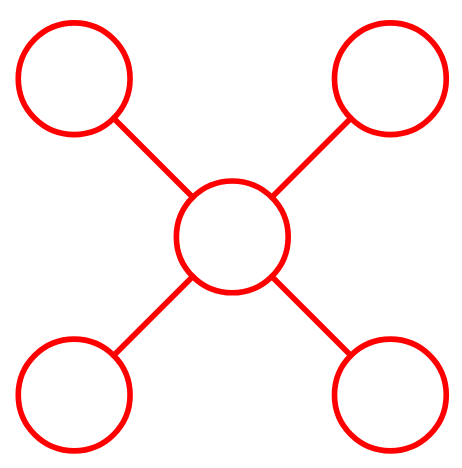
\includegraphics[height=3.5cm]{InferenceTrees1}\\
        Undirected trees.
      \end{center}
    \end{minipage}
    \hspace{0.01\linewidth}
    \begin{minipage}{0.3\linewidth}
      \begin{center}
        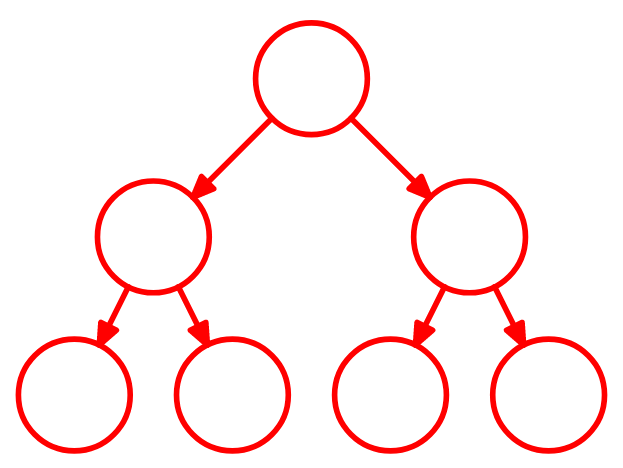
\includegraphics[width=\linewidth]{InferenceTrees2}\\
        Directed trees.
      \end{center}
    \end{minipage}
    \hspace{0.01\linewidth}
    \begin{minipage}{0.3\linewidth}
      \begin{center}
        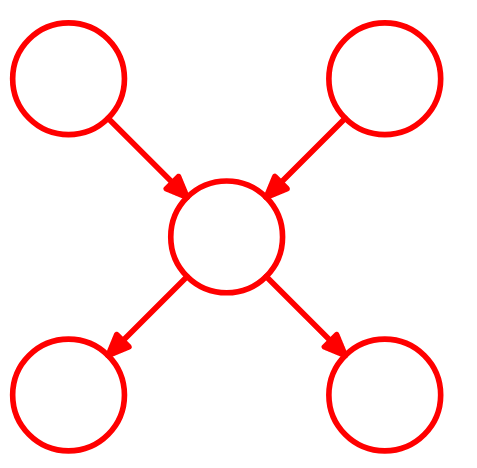
\includegraphics[height=3.5cm]{InferenceTrees3}\\
        Directed polytrees.    
      \end{center}
    \end{minipage}
  \end{center}
\end{minipage}\\
\vspace{0.3cm}
Since explaining these structures per se is quite troublesome, we are introducing \textbf{facto graphs}.
%
%
\subsection{Inference -- Factor Graph}
Factor graphs are an alternative graphical representation which is useful to better explain inference algorithms. \newline
A factor graph is a graphical representation of a graphical model highlighting its factorization, i.e., its conditional probabilities. A factor graph has one node for each node in the original graph, one additional node for each factor (evidence) and undirected links to each of the node variables in the factor. \newline
Mind that each node factor needs to be linked to all the nodes from which the decomposition comes from. \newline
Let's consider for example the following probability distribution:
\[P(X_3\vert X_1,X_2)P(X_1)P(X_2)\]
We know that a Bayesian Network representation can be:
\begin{center}
  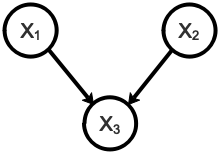
\includegraphics[scale=0.3]{FactorGraphExample1_1}
\end{center}
We could notice that actually $X_3$ is conditioned on $X_1$ and $X_2$ and hence we could create a factor node $f$ as follows:
\begin{center}
  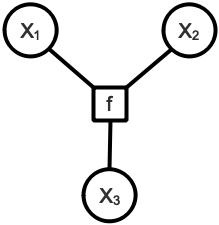
\includegraphics[scale=0.3]{FactorGraphExample1_2}
\end{center}
Actually $f$ can be thought as a function:
\[f(X_1,X_2,X_3)=P(X_3\vert X_1,X_2)P(X_1)P(X_2)\]
Now then it's possible to add also other two factor nodes which would express the probability of the nodes $X_1$ and $X_2$. 
\[f_c(X_1,X_2,X_3)=P(X_3\vert X_1,X_2)\]
\[f_a(X_1)=P(X_1)\]
\[f_b(X_2)=P(X_2)\]
\begin{center}
  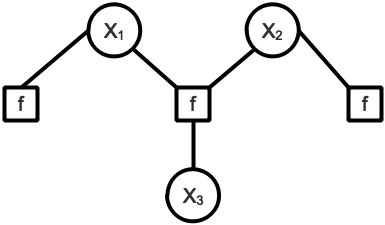
\includegraphics[scale=0.3]{FactorGraphExample1_3}
\end{center}
%
%
\subsection{Sum-Product Algorithm}
The sum-product algorithm is an efficient algorithm for exact inference on tree-structured graphs. As the version for the chains, also this is a message passing algorithm. \newline
This algorithm is applicable to undirected models, i.e., Markov Networks, as well as directed ones, i.e., Bayesian Networks. 
We will now present it on factor graphs assuming a tree-structured graph giving rise to a factor graph which is a tree. \newline
%
\subsubsection{Computing Marginals}
To compute the probability of a single variable, one sums over the probabilities of all variables except the one for which they wish to compute the marginal. \newline
\[P(X)=\Sum_{\vect{X}\setminus X}P(\vect{X})\]
Since $X$ is a node, then the probability $P(X)$ of an event is the product of all the incoming messages from the neighbouring factors $f_s$:
\[P(X)=\Prod_{f_s\in \neigh(X)}\mu_{f_s\rightarrow X}(X)\]
where $\neigh(X)$ are the neighbours of $X$.
\begin{center}
  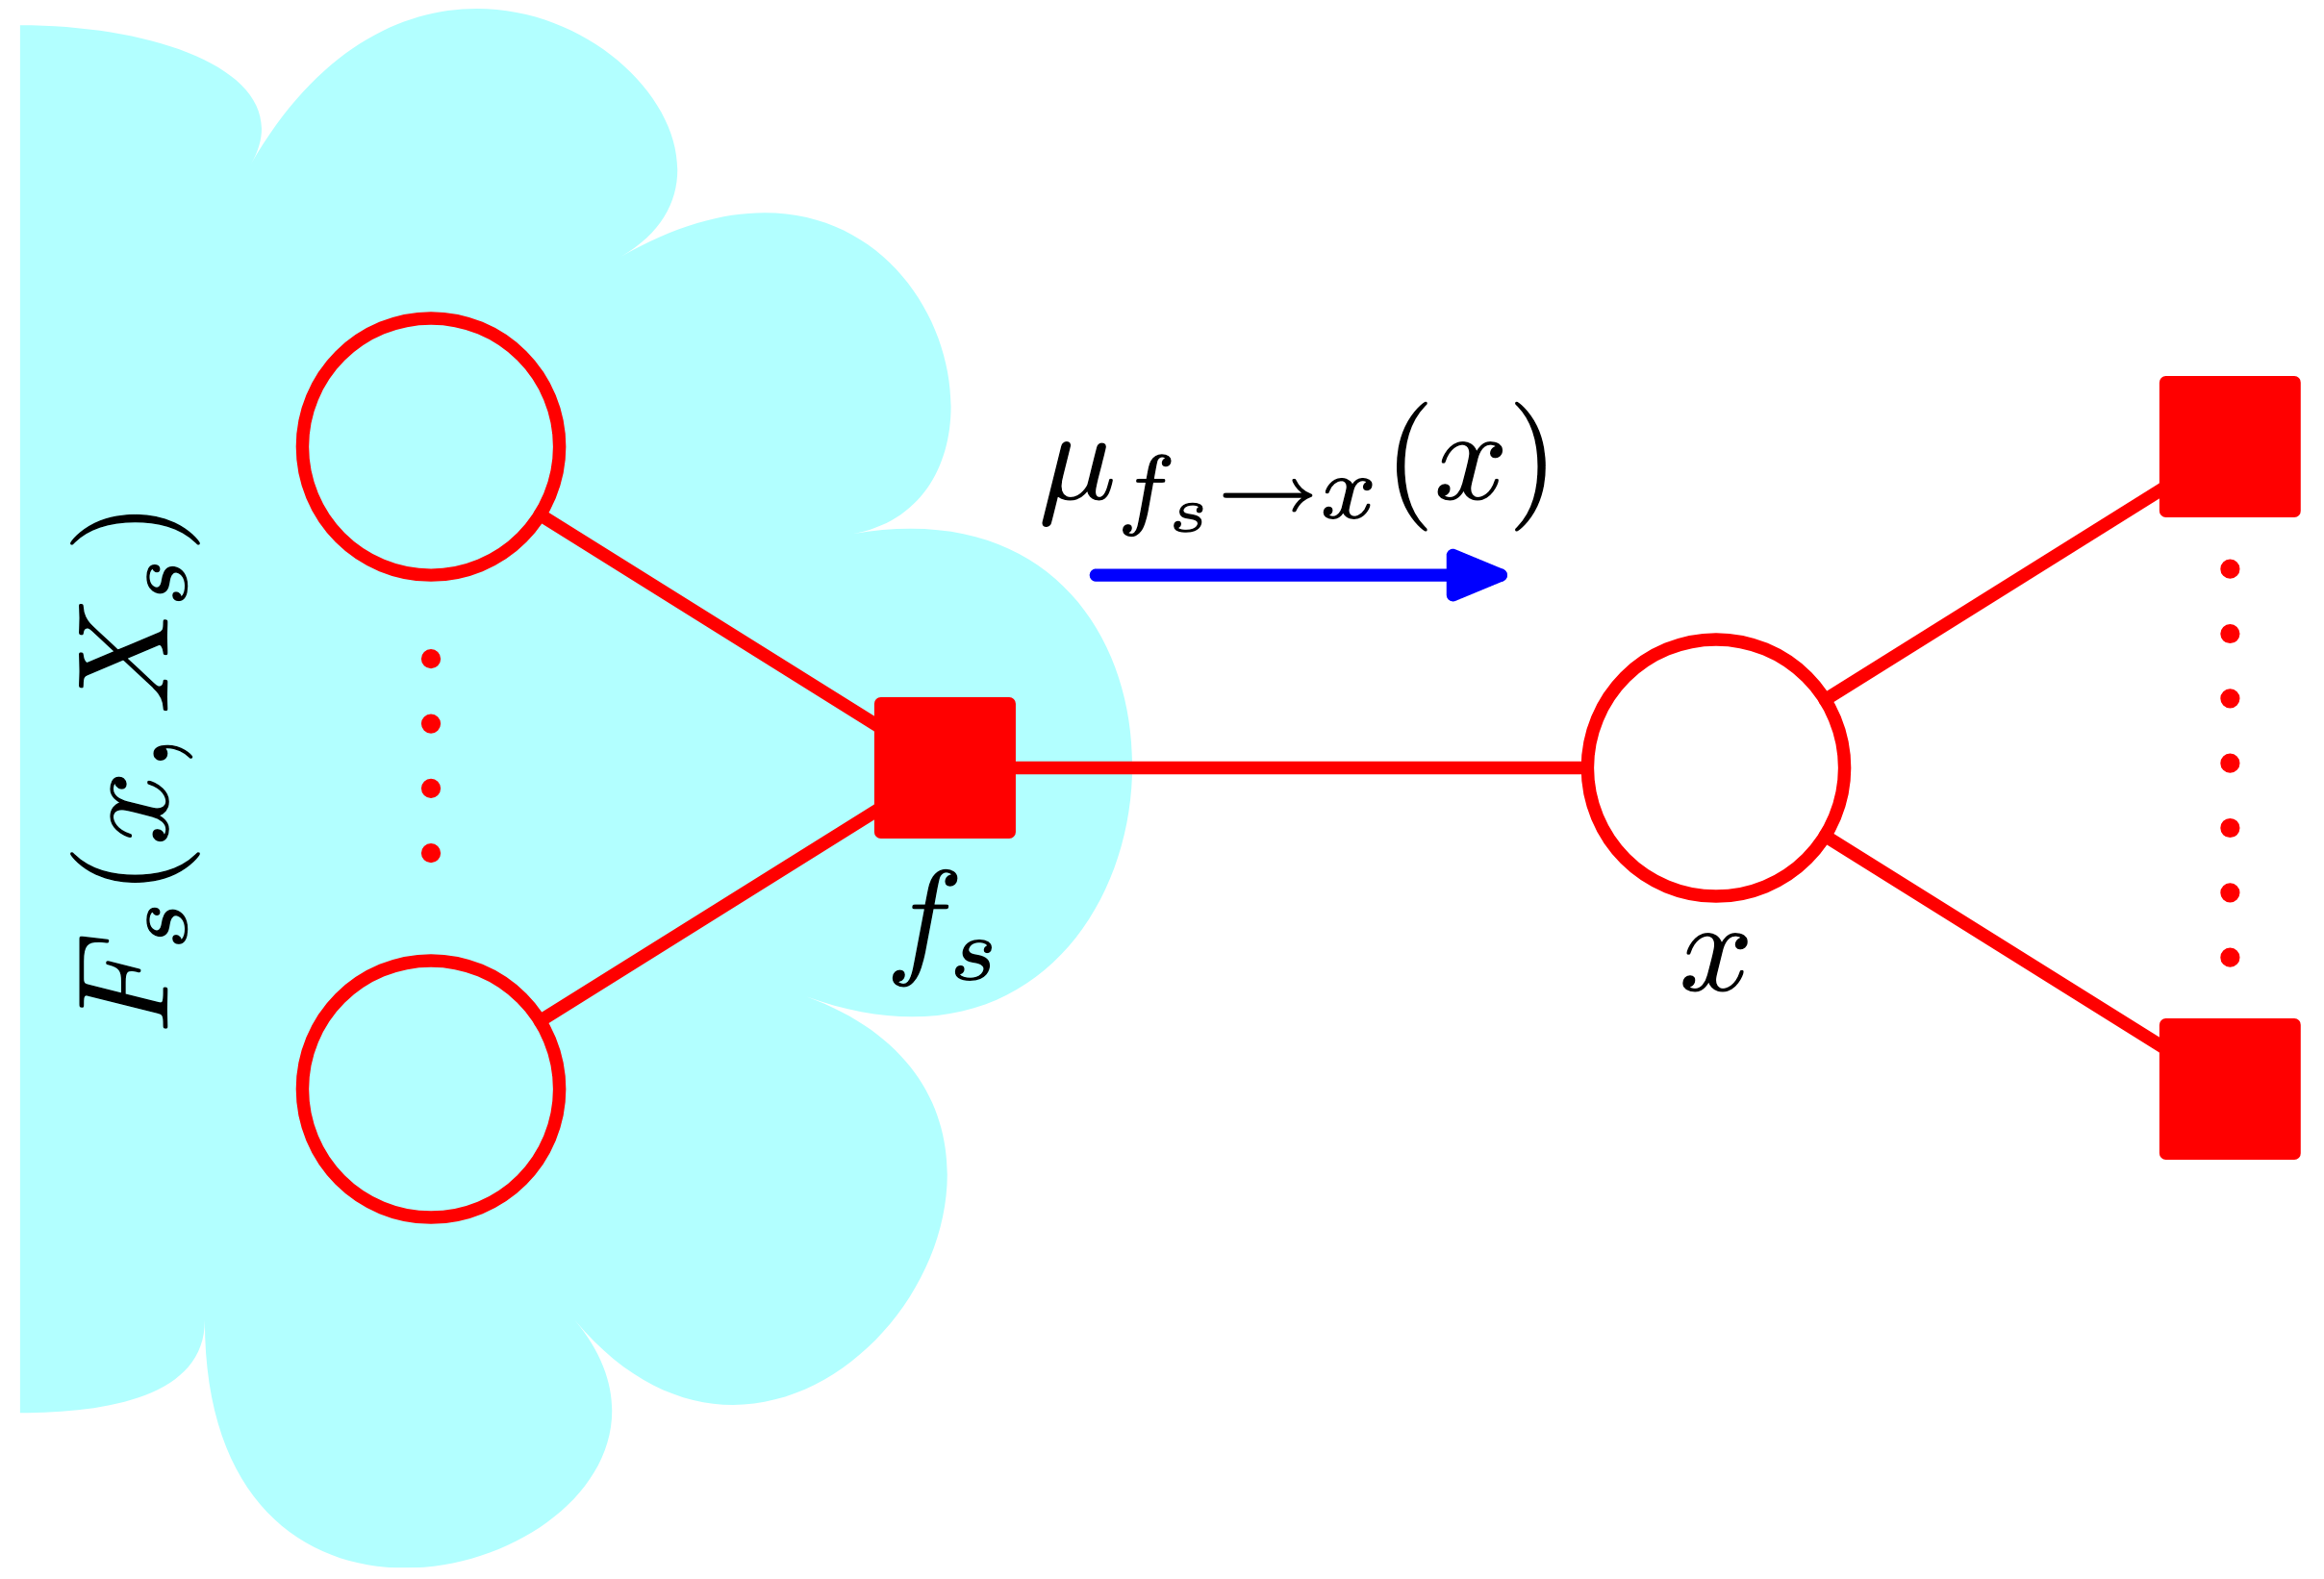
\includegraphics[width=0.5\linewidth]{FactorGraphInference1_1}
\end{center}
Each factor message is the product of messages coming from nodes other than $X$, times the factor, summed over all possible values of the factor variables other than $X$:
\[\mu_{f_s\rightarrow X}(X)=\Sum_{X_1}\hdots\Sum_{X_M} f_s(X,X_1,\hdots,X_M)\Prod_{X_m\in\neigh(f_s)\setminus X}\mu_{X_m\rightarrow f_s}(X_m)\]
\begin{center}
  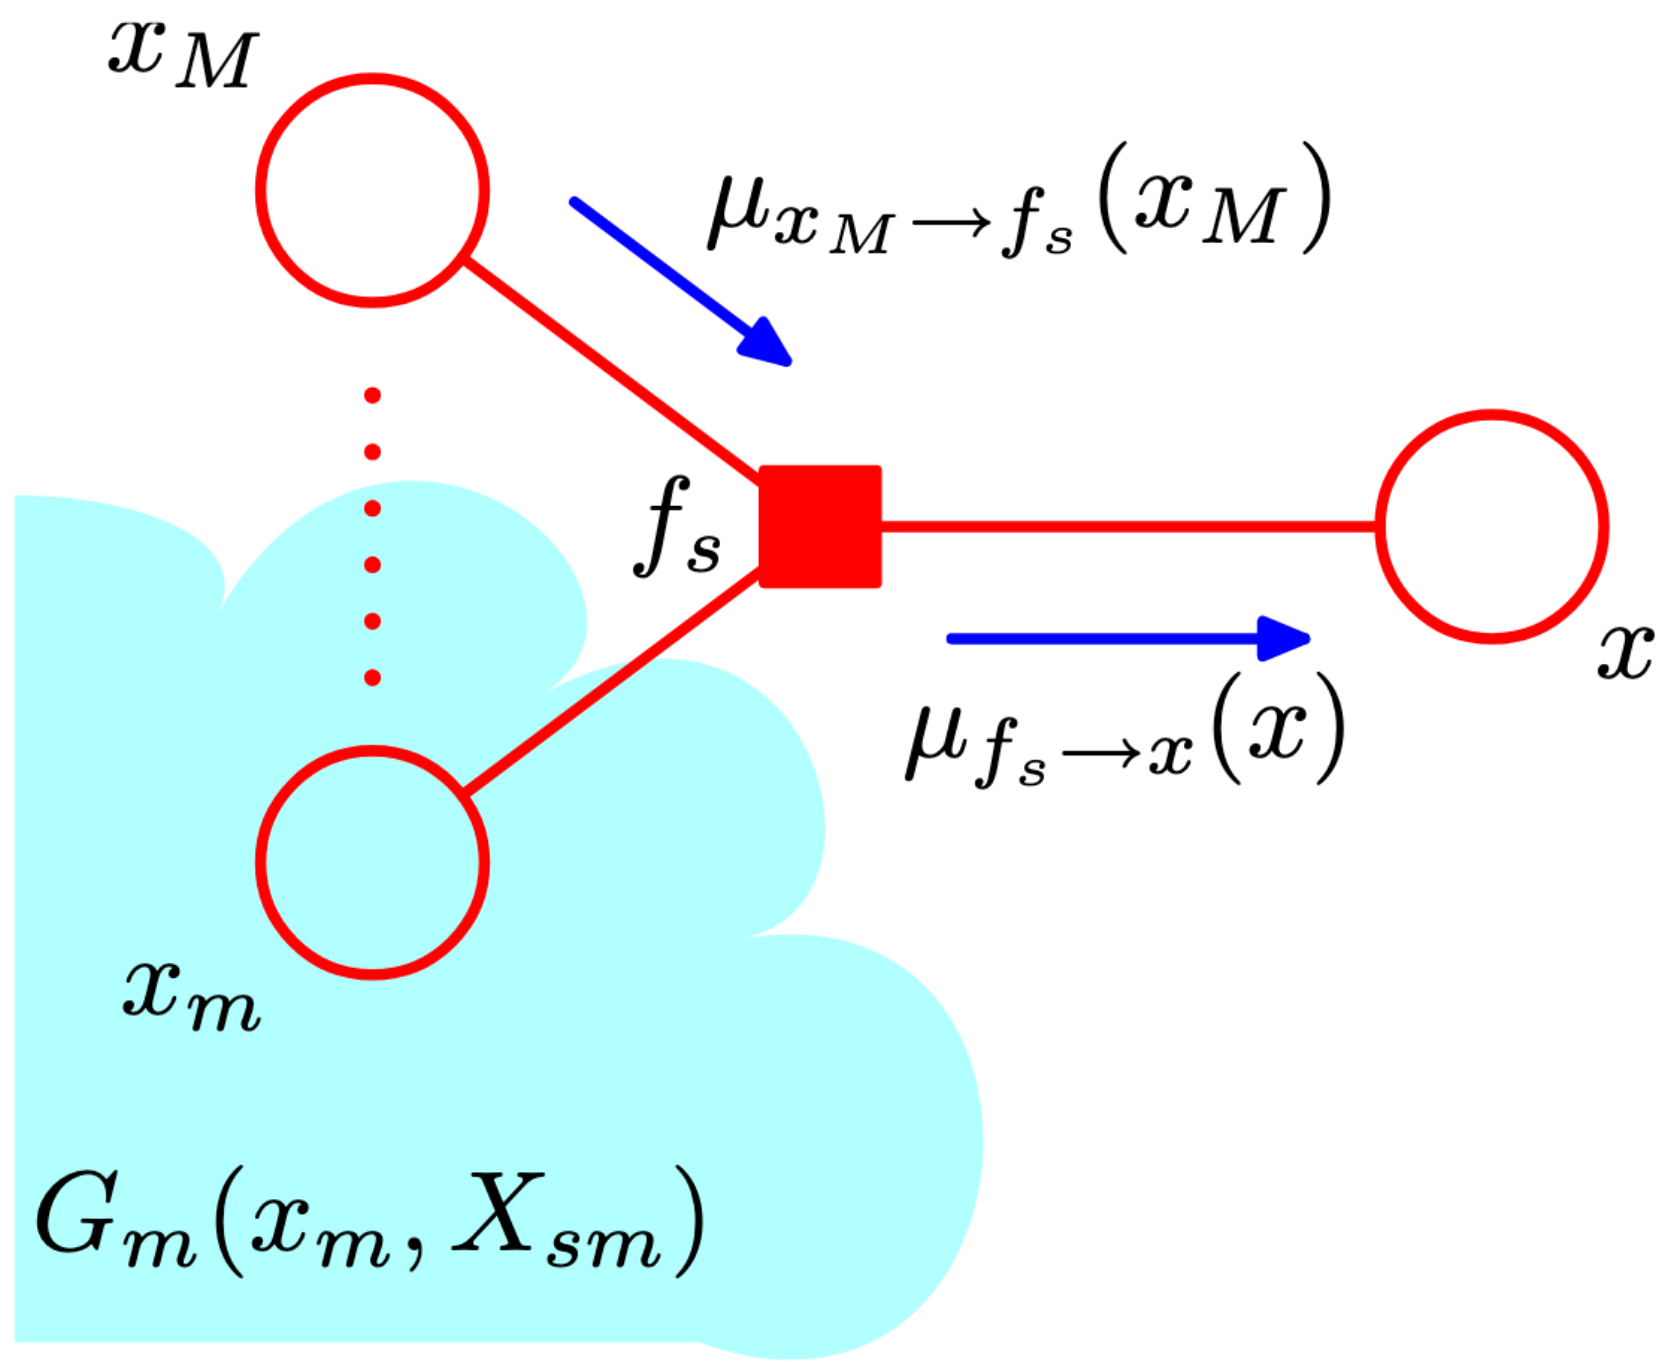
\includegraphics[width=0.5\linewidth]{FactorGraphInference1_2}
\end{center}
Now it's possible to notice that each message from node $X_m$ to factor $f_s$ is the product of the factor message to $X_m$ coming from factors other than $f_s$:
\[\mu_{X_m\rightarrow f_s}(X_m)=\Prod_{f_l\in\neigh(X_m)\setminus f_s}\mu_{f_l\rightarrow X_m}(X_m)\]
\begin{center}
  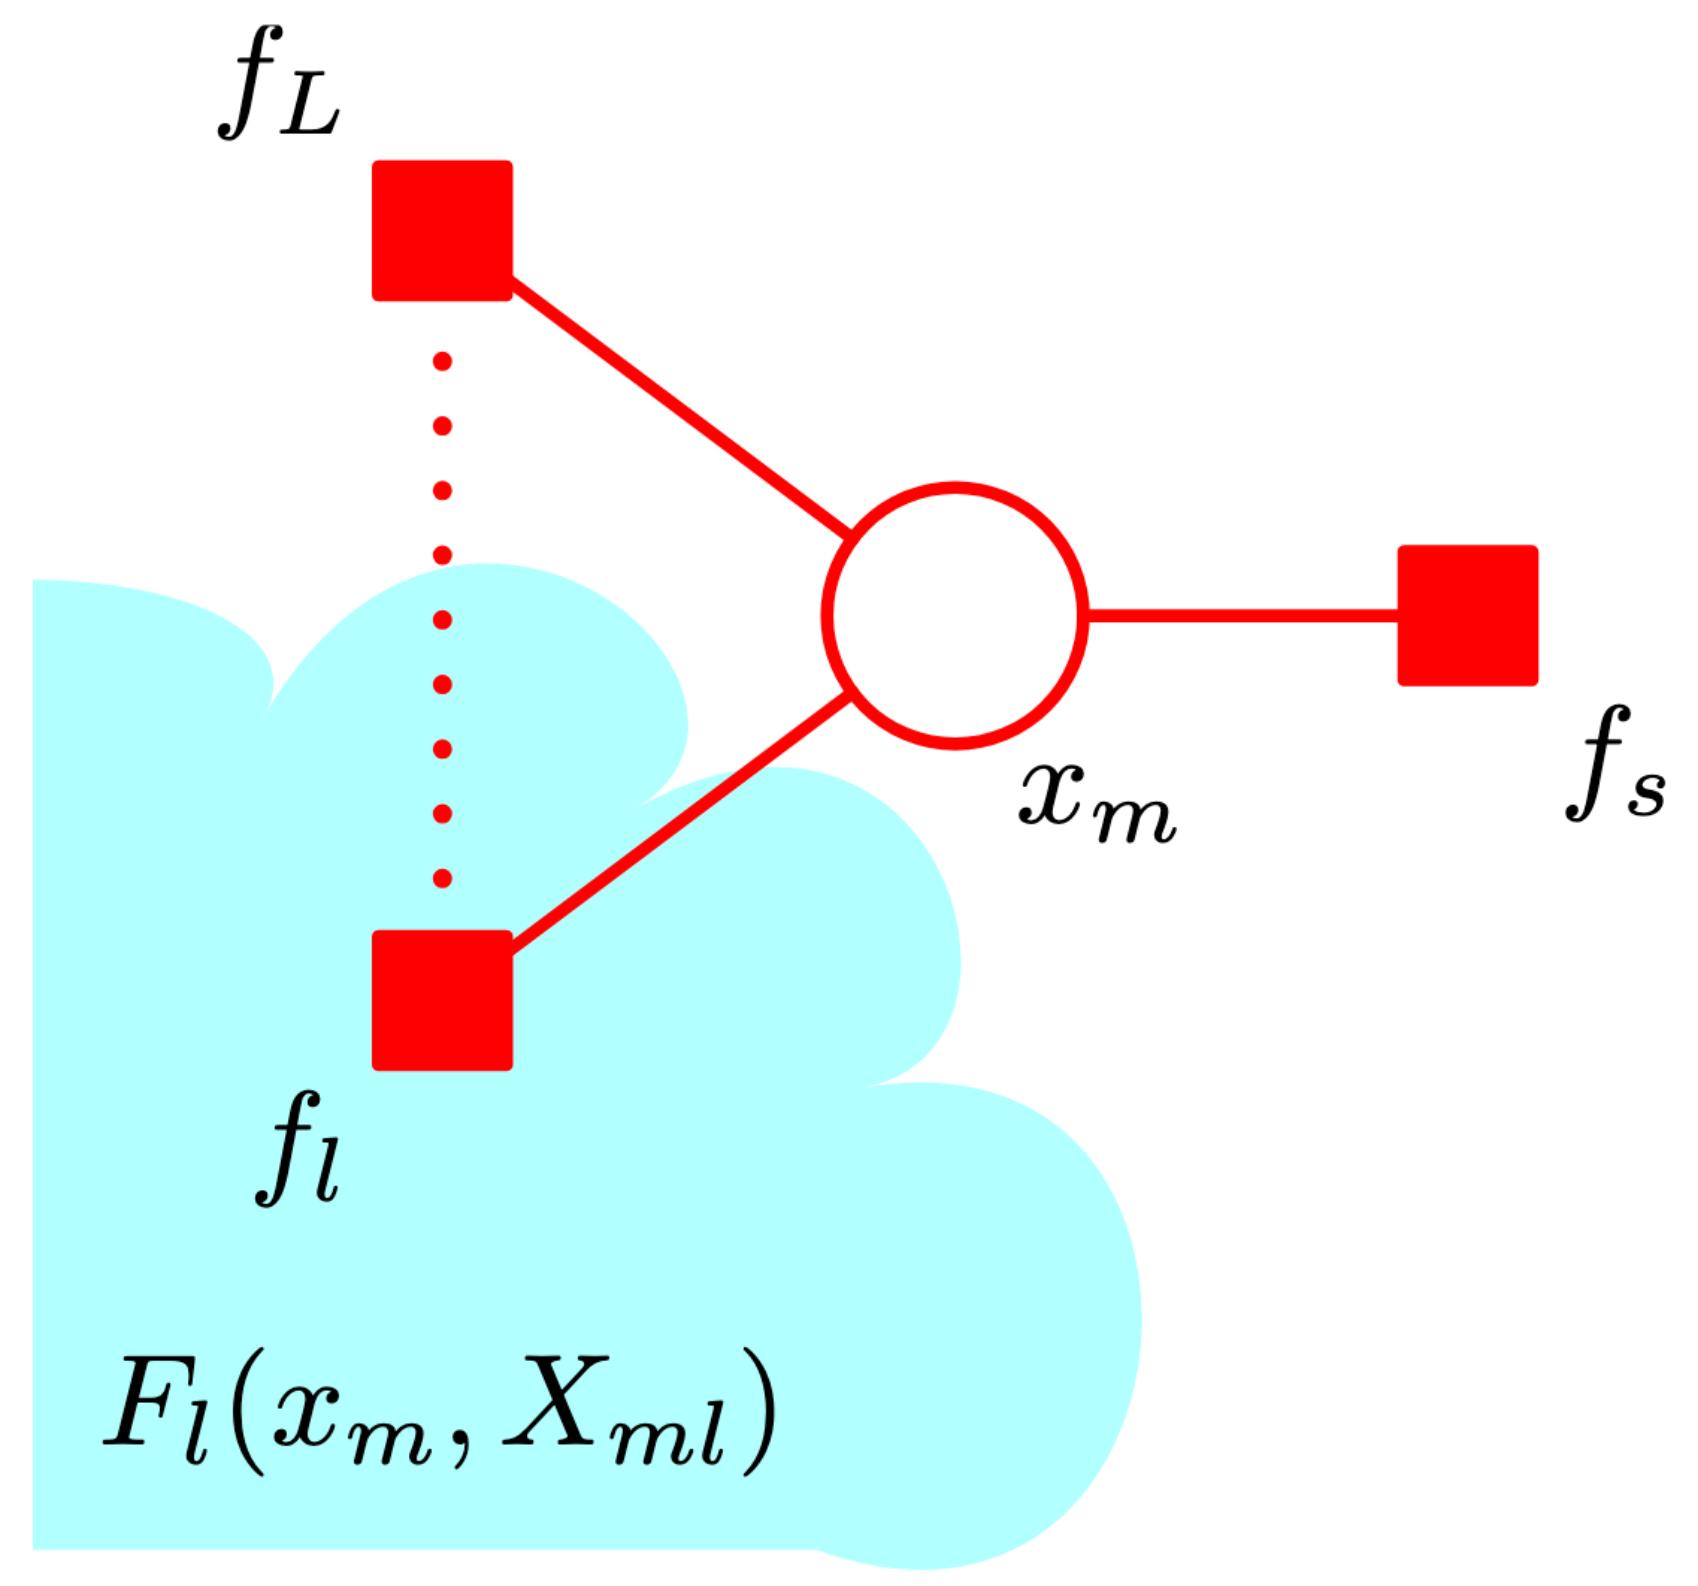
\includegraphics[width=0.5\linewidth]{FactorGraphInference1_3}
\end{center}
Knowing these informations, we can move to the algorithm. First of all the message passing starts from the leaves, either factors or nodes. \newline
If the leaf is a factor, the message is initialized to the factor itself, indeed there would be no $X_m$ different from the destination on which to sum over:
\[\mu_{f\rightarrow x}(x)=f(x)\]
If the leaf is a node, the message is initialized to 1:
\[\mu_{x\rightarrow f}(x)=1\]
Now the node $X$ whose marginal has to be computed is designed as root. Messages are sent from all leaves to their neighbours. Each internal node sends its message towards the root as soon as it has received the messages from all the other neighbours. Once the root has collected all messages, the marginal can be computed as the product of them. 
\begin{center}
  \begin{minipage}[htp]{\linewidth}
    \begin{minipage}[t]{0.48\linewidth}
      \begin{center}
        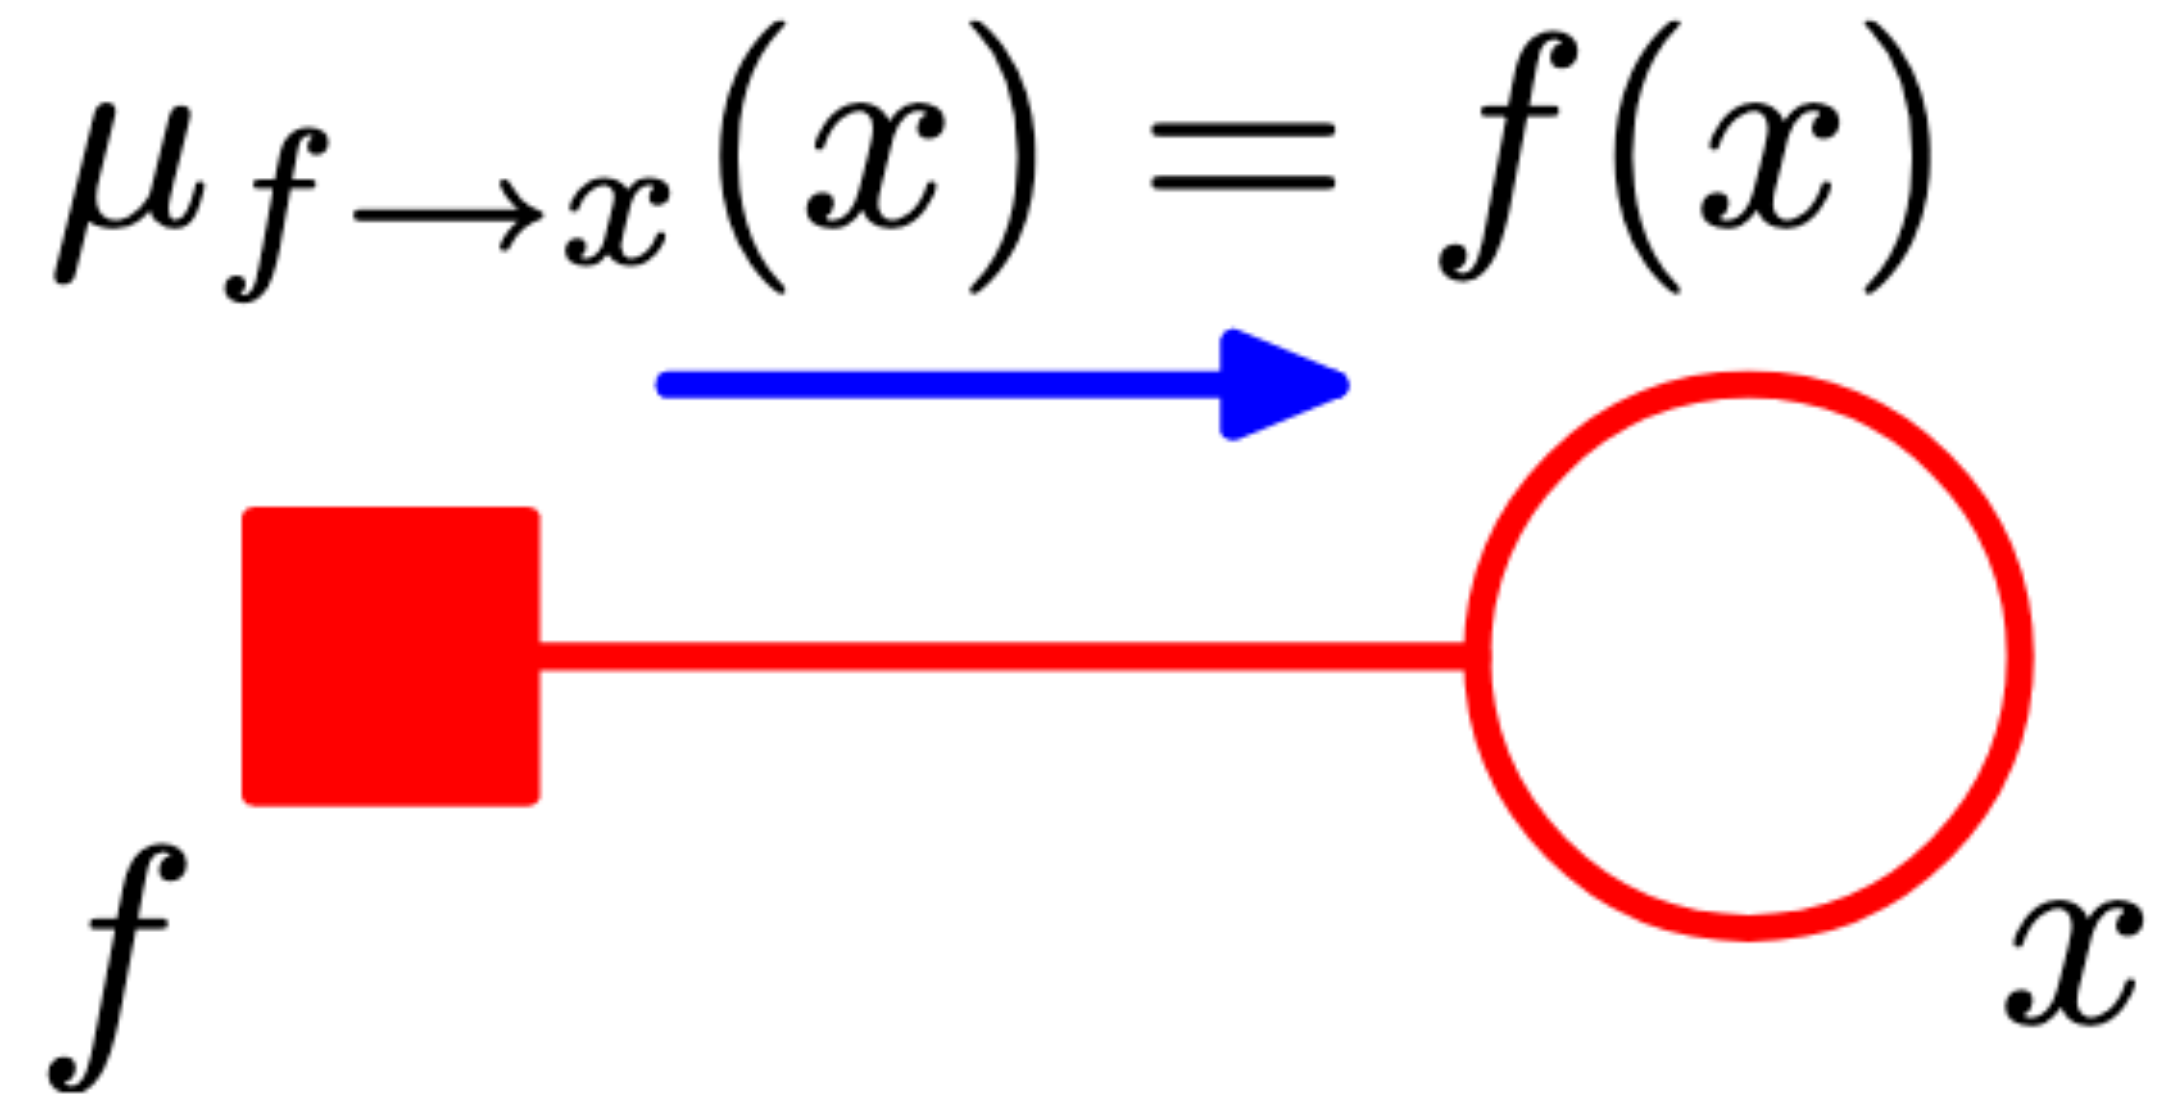
\includegraphics[width=0.6\linewidth]{FactorGraphInference1_4}\\
      \end{center}
      If the leaf is a factor, then the message is initialized to the factor itself.
    \end{minipage}
    \hspace{0.02\linewidth}
    \begin{minipage}[t]{0.48\linewidth}
      \begin{center}
        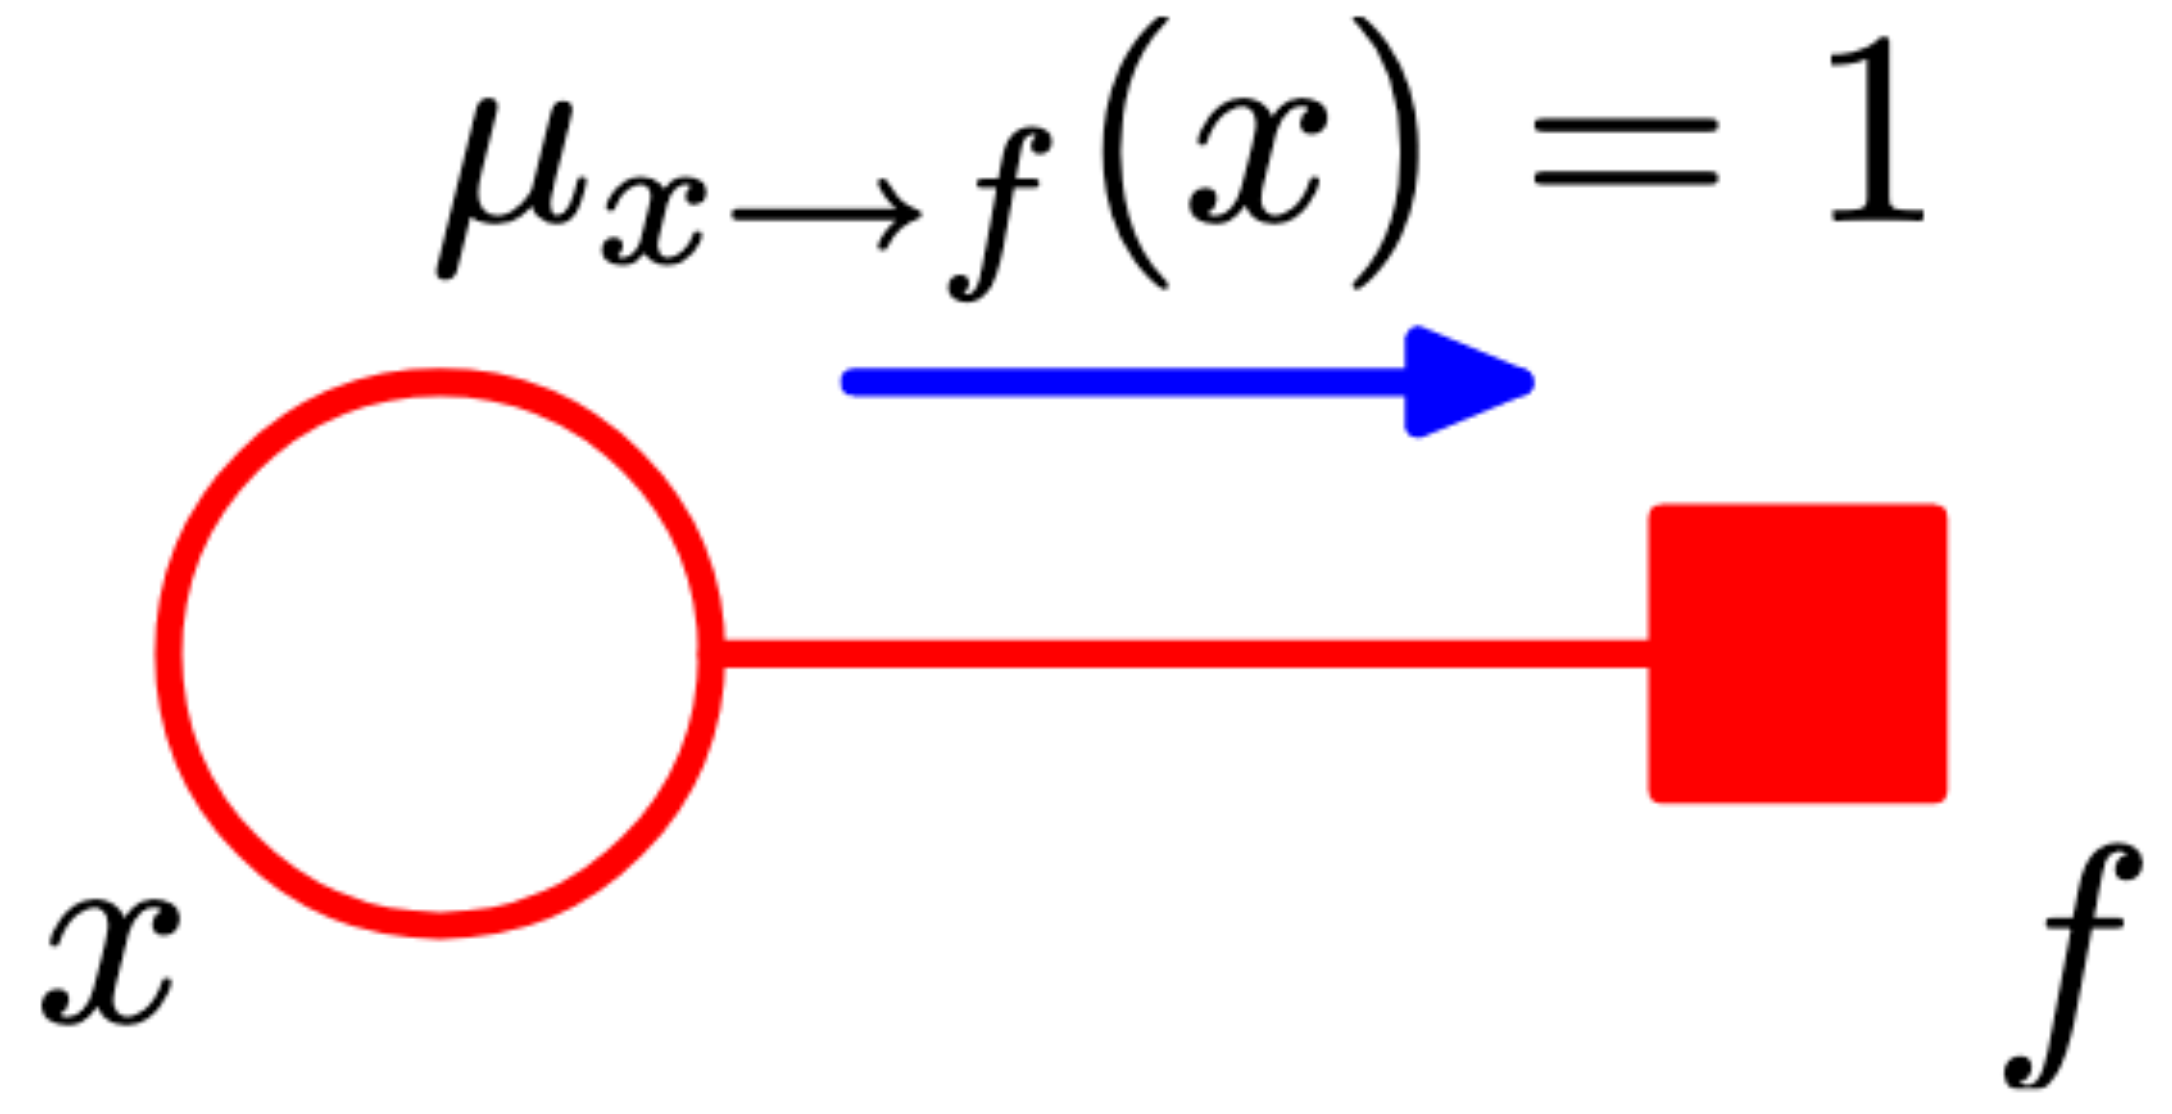
\includegraphics[width=0.6\linewidth]{FactorGraphInference1_5}\\
      \end{center}
      If the leaf is a node, then the message is initialized to 1.
    \end{minipage}
  \end{minipage}
\end{center}
One should remember that for the chain structure the best approach was to send a message from one end to the other and another one on the opposite direction. Similarly, this can be done also for a tree structure: once the root as computed the marginal, send the value back to all the leaves. This allows to pass all messages in all directions using only twice the number of computations used for a single marginal. 
%
\subsubsection{Example}
Let's consider the following factor graph: 
\begin{center}
  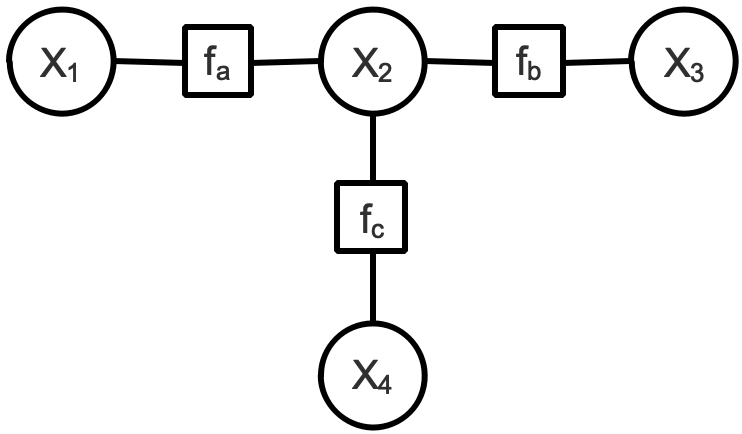
\includegraphics[width=0.7\linewidth]{FactorGraphExample2}
\end{center}
Which has the following joint distribution: 
\[P(\vect{X})=f_a(X_1,X_2)f_b(X_2,X_3)f_c(X_2,X_4)\]
Let's consider the case in which we choose $X_3$ has the root of the tree, hence $X_1$ and $X_4$ are the leafs. Since they are nodes, then the messages are initialized to 1:
\[\mu_{X_1\rightarrow f_a}(X_1)=1\]
\[\mu_{X_4\rightarrow f_c}(X_4)=1\]
By definition, the message from factors to nodes is the product of the messages coming from nodes other then $X_i$, times the factor, summed over all possible values of the factor variables other than $X_i$. Since for both factors $f_a$ and $f_c$ there is only one node before, hence one single message which value is 1, then it's possible to write:
\[\mu_{f_a\rightarrow X_2}(X_2)=\Sum_{X_1}f_a(X_1,X_2)\]
\[\mu_{f_c\rightarrow X_2}(X_2)=\Sum_{X_4}f_a(X_2,X_4)\]
Now we need to send a message from the node $X_2$ to the factor $f_b$, and by definition, such message is the product of the message arriving to $X_2$:
\[\mu_{X_2\rightarrow f_b}(X_2)=\mu_{f_a\rightarrow X_2}(X_2)\mu_{f_c\rightarrow X_2}(X_2)\]
Then the message from $f_b$ to $X_3$ can be written as:
\[\mu_{f_b\rightarrow X_3}(X_3)=\Sum_{X_2}f_b(X_2,X_3)\mu_{X_2\rightarrow f_b}(X_2)\]
Now we need to do the opposite, that is, start from $X_3$ and go towards the leaves. Since $X_3$ is a node, then the message is initialized to 1:
\[\msg{X_3}{f_b}{X_3}=1\]
From factor $f_b$ to factor node $X_2$ we have:
\[\msg{f_b}{X_2}{X_2}=\Sum_{X_3}f_b(X_2, X_3)\]
From $X_2$ to factors $f_a$ and $f_c$:
\[\msg{X_2}{f_a}{X_2})=\msg{f_b}{X_2}{X_2}\msg{f_c}{X_2}{X_2}\]
\[\msg{X_2}{f_c}{X_2})=\msg{f_b}{X_2}{X_2}\msg{f_a}{X_2}{X_2}\]
Finally the message to the leaves are:
\[\msg{f_a}{X_1}{X_1})=\Sum_{X_2}f_a(X_1, X_2)\msg{X_2}{f_a}{X_2}\]
\[\msg{f_c}{X_4}{X_4})=\Sum_{X_2}f_c(X_2, X_4)\msg{X_2}{f_c}{X_2}\]
Now that we have all the information that we need, we could for example decide to compute the marginal probability of $X_2$. We know that the marginal can be computed as the product of all the incoming messages:
\[P(\vect{X})=\msg{f_a}{X_2}{X_2}\msg{f_b}{X_2}{X_2}\msg{f_c}{X_2}{X_2}\]
By expanding each message as written before, we obtain:
\[=\left[\Sum_{X_1}f_a(X_1, X_2)\right]\left[\Sum_{X_3}f_b(X_2, X_3)\right]\left[\Sum_{X_4}f_c(X_2, X_4)\right]\]
\[=\Sum_{X_1}\Sum_{X-3}\Sum_{X_4}f_a(X_1,X_2)f_b(X_2,X_3)f_c(X_2,X_4)\]
But the product of all factors is nothing but the initial distribution:
\[=\Sum_{X_1}\Sum_{X-3}\Sum_{X_4}P(\vect{X})\]
This "proves" that we could use just two passing of messages to compute the marginal probabilities. \newline
%
\subsubsection{Example -- Adding Evidence}
As said before, if any node is observed, then we simply use their observed values instead of summing over all possible values when computing their messages. After normalization this gives the conditional probability given the evidence. \newline
Consider for example the following probability distribution:
\[P(B\vert A,C)P(A)P(C\vert D)P(D)\]
Let's now represent this via a Bayesian Network:
\begin{center}
  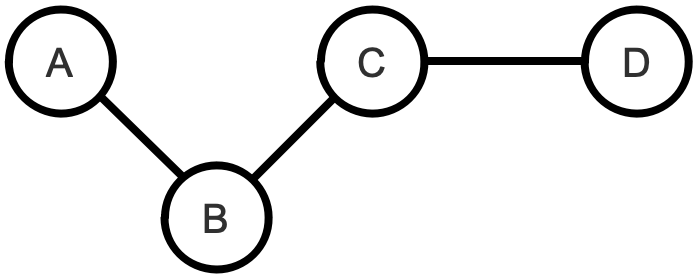
\includegraphics[width=0.5\linewidth]{FactorGraphExample3_1}
\end{center}
We could convert it to a factor graph by looking at its probability distribution and adding a function for each probability:
\begin{center}
  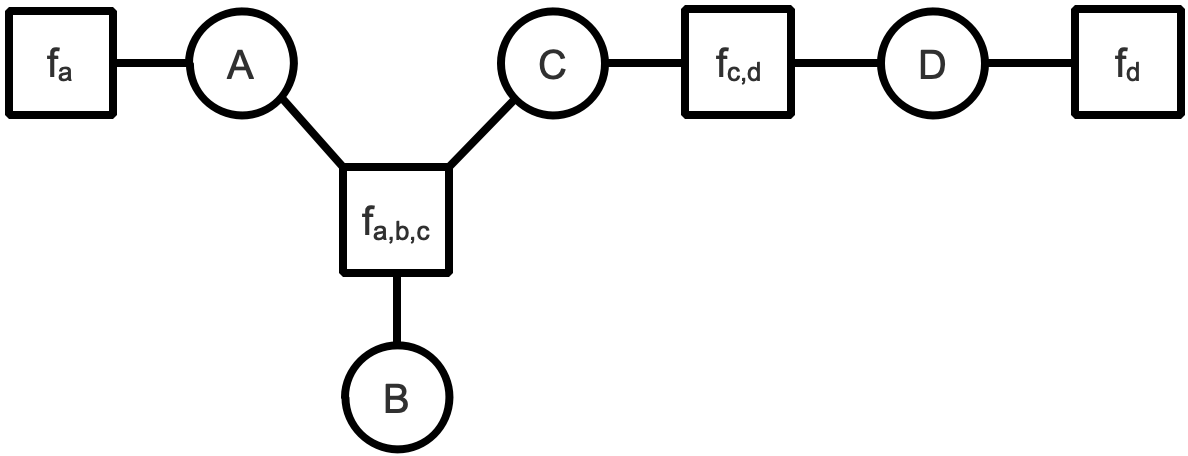
\includegraphics[width=0.6\linewidth]{FactorGraphExample3_2}
\end{center}
Let's consider the case in which we'd like to compute the marginal of $B$. Notice that when we know which node we want to compute the probability of, then we can just use one passage of messages. So let's make $B$ the root of the tree and start from $f_a$ and $f_d$ which are the leaves. Since the leaves are factors, then we can use directly their probability:
\[\mu_{f_A\rightarrow A}=P(A)\]
\[\mu_{f_D\rightarrow D}=P(D)\]
This are the incoming messages to $A$ and $D$ respectively. Now let's compute the outgoing messages; since both $A$ and $B$ do not have any factor except for $f_A$ and $f_D$ respectively, then their messages are:
\[\msg{A}{f_{A,B,C}}{A}=\mu_{f_A\rightarrow A}=P(A)\]
\[\msg{D}{f_{C,D}}{D}=\mu_{f_D\rightarrow D}=P(D)\]
Now let's wait for the branch of $A$ and focus on the branch of $C$ and $D$. We'll send a message from factor $f_{C,D}$ to node $C$. In this case we'll have to sum over all possible values of $D$: 
\[\msg{f_{C,D}}{C}{C}=\Sum_{D}P(C\vert D)\msg{D}{f_{C,D}}{D}=\Sum_DP(C\vert D)P(D)\]
We can now also send the message from $C$ to factor $f_{A,B,C}$:
\[\msg{C}{f_{A,B,C}}{C}=\msg{f_{C,D}}{C}{C}=\Sum_DP(C\vert D)P(D)\]
At last the factor $f_{A,B,C}$ sends a message to the node $B$:
\[
  \begin{array}{ll}
    \msg{f_{A,B,C}}{B}{B}&=\Sum_A\Sum_CP(B\vert A,C)\msg{C}{f_{A,B,C}}{C}\msg{A}{f_{A,B,C}}{A}\\
                         &=\Sum_A\Sum_CP(B\vert A,C)P(A)\Sum_DP(C\vert D)P(D)
  \end{array}
\]
Since the marginal probability of a node is the product of all incoming messages to the node, we have:
\[
  \begin{array}{ll}
    P(B)=\msg{f_{A,B,C}}{B}{B}&=\Sum_A\Sum_CP(B\vert A,C)P(A)\Sum_DP(C\vert D)P(D)\\
                              &=\Sum_A\Sum_C\Sum_DP(B\vert A, C)P(A)P(C\vert D)P(D)\\
                              &=\Sum_A\Sum_C\Sum_DP(A,B,C,D)
  \end{array}
\]
%
\subsection{Most Probable Configuration}
Consider the following case: we are given a joint probability distribution $p(\vect{X})$ and our goal is to find the configuration for variables $\vect{X}$ having the highest probability:
\[\vect{X}^{\text{max}}=\argmax{\vect{X}}P(\vect{X})\]
for which the probability is:
\[P(\vect{X}^{\text{max}})=\max\limits_{\vect{X}}P(\vect{X})\]
For instance, we are not interested in computing the probability that in the next days it'll rain, but in knowing which is the most probable weather during the next week. \newline
Notice that we are trying to find the configuration which is jointly maximal for all variables, that is if the variables are not independent, we cannot simply compute $P(X_i)$ for each $i$ and then maximize. \newline
As for the sum-product algorithm, we can exploit the distribution factorization to efficiently compute the maximum:
\[P(\vect{X}^{\text{max}})=\max\limits_{\vect{X}}P(\vect{X})=\max\limits_{X_1}\hdots\max\limits_{X_M}P(\vect{X})\]
All we have done is to replace the sum from the sum-product algorithm with a $\max$ function. When doing these maximizations, we are actually ignoring all the variables that are not the variable we are trying to maximize.
%
\subsubsection{Chain Example}
Let's consider a simple chain:
\begin{center}
  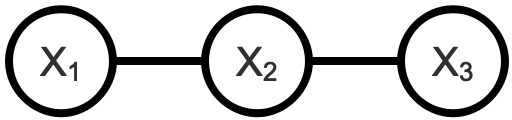
\includegraphics[width=0.5\linewidth]{MPCExample1}
\end{center}
And let's say that the variables can take the following values: $X_1=\{\text{Rainy, Cloudy, Sunny}\},~ X_2=\{T,F\},~ X_3=\{T,F\}$. The probability for $X_1$ and the conditional probabilities are the following:
\begin{center}
  \begin{tabular}{cc|c|}
    \cline{3-3}
    \multirow{3}{*}{$X_1$}&R&0.2\\
    \cline{3-3}
                          &C&0.2\\
    \cline{3-3}
                          &S&0.6\\
    \cline{3-3}
  \end{tabular}
  \hspace{1cm}
  \begin{tabular}{C{0.2cm}c}
          &$X_1$\\
    $X_2$&
      \begin{tabular}{c|c|c|c|}
        \mc{1}{c}{}&\mc{1}{c}{R}&\mc{1}{c}{C}&\mc{1}{c}{S}\\
        \cline{2-4}
        T&0.2&0.4&0.8\\
        \cline{2-4}
        F&0.8&0.6&0.2\\
        \cline{2-4}
      \end{tabular}
  \end{tabular}
  \hspace{1cm}
  \begin{tabular}{C{0.2cm}c}
          &$X_2$\\
    $X_3$&
      \begin{tabular}{c|c|c|}
        \mc{1}{c}{}&\mc{1}{c}{T}&\mc{1}{c}{F}\\
        \cline{2-3}
        T&0.8&0.4\\
        \cline{2-3}
        F&0.2&0.6\\
        \cline{2-3}
      \end{tabular}
  \end{tabular}
\end{center}
The joint probability of a chain is:
\[P(\vect{X})=P(X_3\vert X_2)P(X_2\vert X_1)P(X_1)\]
Our goal is to find the values for $X_1,X_2,X_3$ that maximize the joint probability. \newline
Each maximization can be seen as an outgoing message ($\mu_\beta$) where instead of having a sum we are actually maximizing. For instance:
\[\mu_\beta(X_2)=\max\limits_{X_3}P(X_3\vert X_2)=
  \begin{cases}
    \begin{array}{ll}
      0.8&\text{if }X_2=T\\
      0.6&\text{if }X_2=F\\
    \end{array}
  \end{cases}
\]
The result is due to the fact that, looking at the rightmost table, fixating a value for $X_2$, it's possible to find the maximum probability, for instance, if $X_2$ is $T$, then the $P(X_3=T\vert X_2=T)>P(X_3=F\vert X_2=T)$. \newline
The same can be done to compute the value for $X_2$:
\[\mu_\beta(X_1)=\max\limits_{X_2}P(X_2\vert X_1)\mu_\beta(X_2)=
\begin{cases}
  \begin{array}{ll}
    0.48&\text{if }X_1=R\\
    0.36&\text{if }X_1=C\\
    0.64&\text{if }X_1=S
  \end{array}
\end{cases}
\]
In order to compute this we have to look at the center table above. First let's consider the case in which $X_1=R$, then we could have $P(X_1=R\vert X_2=T)=0.2$, or $P(X_1=R\vert X_2=F)=0.8$. We want to check both of these possibilities and take the highest value:
\[P(X_1=R\vert X_2=T)\mu_\beta(X_2=T)=0.2\cdot 0.8=0.16\]
\[P(X_1=R\vert X_2=F)\mu_\beta(X_2=F)=0.8\cdot 0.6=0.48\]
Then we choose the highest value, that is $0.48$. The same reasoning is applied for $P(X_1=C\vert X_2)$ and $P(X_1=S\vert X_2)$
\[P(X_1=C\vert X_2=T)\mu_\beta(X_2=T)=0.4\cdot 0.8=0.48\]
\[P(X_1=C\vert X_2=F)\mu_\beta(X_2=F)=0.6\cdot 0.6=0.36\]
\[P(X_1=S\vert X_2=T)\mu_\beta(X_2=T)=0.8\cdot 0.8=0.64\]
\[P(X_1=S\vert X_2=F)\mu_\beta(X_2=F)=0.2\cdot 0.6=0.12\]
At last we can compute the maximum configuration probability:
\[P(\vect{X}^{\text{max}})=\max\limits_{X_1}P(X_1)\mu_\beta(X_1)=\max\limits_{X_1}
  \begin{bmatrix}
    0.48\cdot 0.2\\
    0.36\cdot 0.2\\
    0.64\cdot 0.6
  \end{bmatrix}
  =0.64\cdot 0.6=0.384
\]
The most likely configuration for $X_1$ is:
\[\argmax{X_1}P(X_1)\mu_\beta(X_1)=S\]
Then to know the most likely configuration for $X_2$ all we need to do is to go back to the computation of $\mu_\beta(X_1)$ and look to which value gave the highest probability when $X_1=S$, that is when $X_2=T$, $P(X_1=S\vert X_2=T)\mu_\beta(X_2)=0.64$. \newline
The same is done for $X_3$ keeping in mind that now we know that $X_2=T$: given such information, the highest probability is obtained for $X_3=T$, $P(X_3=T\vert X_2=T)=0.8$. \newline
This action of retrieving the correct configuration going backwards is called \textbf{backpropagation}. 
%
\subsubsection{Tree}
As we saw in the example before, the max-product algorithm can be seen as a message passing over the graph. The algorithm is thus easily applied to tree-structured graphs via their factor trees: all one needs to do is to change the sum with a maximization:
\[\msg{f}{X}{X}=\max\limits_{X_1,\hdots,X_M}\left[f(X, X_1, \hdots, X_M)\Prod_{X_m\in\neigh(f)\setminus X}\msg{X_m}{f}{X_m}\right]\]
\[\msg{X}{f}{X}=\Prod_{f_l\in\neigh(X)\setminus f}\msg{f_l}{X}{X}\]
As the sum-product algorithm, once a root $X_r$ is chosen, the leaves send messages towards the root. The probaility of the maximal configuration is readily obtained as:
\[P(\vect{X}^{\text{max}})=\max\limits_{X_r}\left[\Prod_{f_l\in\neigh(X_r)}\msg{f_l}{X_r}{X_r}\right]\]
The maximal configuration for the root is obtained as:
\[X_r^{\text{max}}=\argmax{X_r}\left[\Prod_{f_l\in\neigh(X_r)}\msg{f_l}{X_r}{X_r}\right]\]
We now need to recover the maximal configuration for the other variables. When sending a message towards $x$, each factor node should store the configuration of the other variables which gave the maximum:
\[\phi_{f\rightarrow X}(X)=\argmax{X_1,\hdots, X_M}\left[f(X,X_1,\hdots,X_M)\Prod_{X_m\in\neigh(f)\setminus X}\msg{X_m}{f}{X_m}\right]\]
When the maximal configuration for the root node $X_r$ has been obtained, it can be used to retrieve the maximal configuration for the variables in neighbouring factors from:
\[X_1^{\text{max}},\hdots,X_M^{\text{max}}=\phi_{f\rightarrow X_r}\left(X_r^{\text{max}}\right)\]
The procedure can be repeated \textit{back-tracking} to the leaves, retrieving maximal values for all variables. \newline
For the chain we saw before, back-tracking resolves in:
\[
  \begin{array}{lll}
    X_N^{\text{max}}&=&\argmax{X_N}\msg{f_{N-1,N}}{X_N}{X_N}\\
    X_{N-1}^{\text{max}}&=&\phi_{f_{N_1,N}\rightarrow X_N}(X_{N}^{\text{max}})\\
    X_{N-2}^{\text{max}}&=&\phi_{f_{N_2,N-1}\rightarrow X_{N-1}}(X_{N-1}^{\text{max}})\\
                        &\vdots&\\
    X_{1}^{\text{max}}&=&\phi_{f_{1,2}\rightarrow X_2}(X_{2}^{\text{max}})\\
  \end{array}
\]
%
\subsubsection{Trellis}
It's possible to visualize the best configuration by using a trellis diagram which shows the $K$ possible states of each variable $X_n$ one per row. For each state $k$ of a variable $X_n$, $\phi_{f_{n-1, n}\rightarrow X_n}(X_n)$ defines a unique (maximal) previous state, linked by an edge in the diagram. \newline
Once the maximal state for the last variable $X_N$ is chosen, the maximal states for other variables are recovered following the edges backwards. 
\begin{center}
  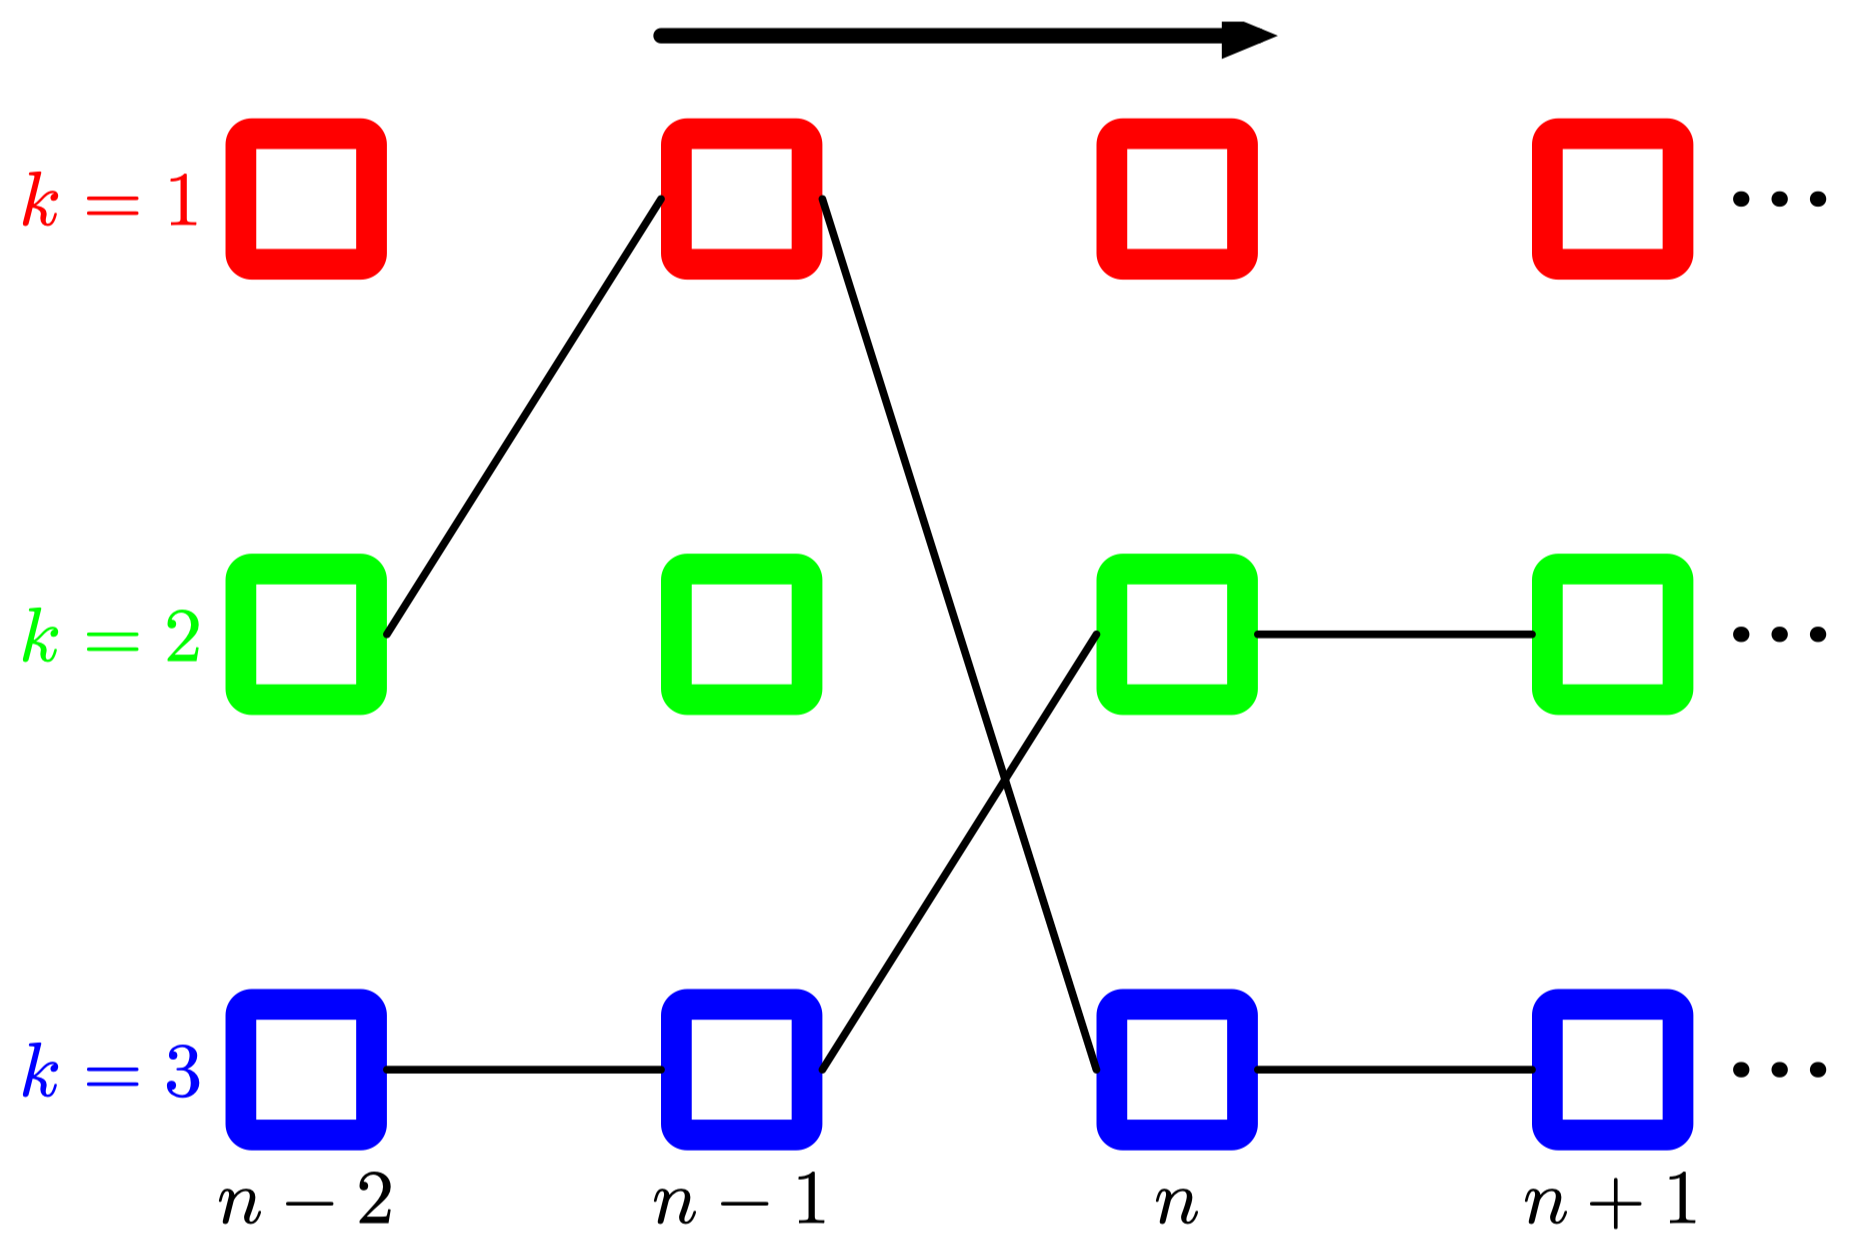
\includegraphics[width=0.6\linewidth]{InferenceTrellis}
\end{center}
\data{30/10/2019}
%
\subsubsection{Underflow}
The max-product algorithm relies on products, but the multiplication of small numbers (probabilities) can lead to underflow problems. This can be solved by considering $\log(\max(P(\vect{X})))$ instead of simply $\max(P(\vect{X}))$. \newline
Since the logarithm is monotonic, we have that the proper maximal configuration is recovered:
\[\log\left(\max\limits_{\vect{X}}P(\vect{X})\right)=\max\limits_{\vect{X}}\log(P(\vect{X}))\]
Moreover we know that, by the properties of logarithms, the multiplication of logarithms can be converted into a sum, giving the \textit{max-sum} algorithm. \newline
%
%
\subsection{Exact Inference -- Junction Tree Algorithm}
Let's see how to deal with inference when the network structure is not as nice as the ones we have seen until now. Indeed many applications require graphs with (undirected loops), so we acutally need an extension of the max-product algorithm to generic graphs. \newline
Such new algorithm is called \textbf{junction tree} algorithm. As the name suggests, this algorithm does not work on factor graphs, but on junction trees, i.e., tree-structured graphs with nodes containing clusters of variables of the original graph. Then a message passing scheme similar to the sum-product and max-product algorithms is run on the junction tree. \newline
Notice though that such an algorithm is exponential on the maximal number of variables in a cluster, making it intractable for large complex graphs. 
%
%
\subsection{Approximate Inference}
If the graph is too large or complex and the junction tree algorithm is not usable, then we can resort to \textit{approximate} techniques such as:
\begin{itemize}
  \item \textit{Loopy belief propagation}: message passing on the original graph even if it contains loops;
  \item \textit{Variational methods}: deterministic approximations, assuming the posterior probability (given the evidence) factorizes in a particular way;
  \item \textit{Sampling methods}: approximate posterior is obtained sampling from the network.
\end{itemize}
%
\subsubsection{Loopy Belief Propagation}
The idea is simply to apply the sum-product algorithm even if it is not guaranteed to provide an exact solution. \newline
We assume all nodes are in condition of sending messages, i.e., they already received a constant 1 message from all neighbours. \newline
A message passing schedule is chosen in order to decide which nodes start sending messages, e.g., flooding. \newline
The information than flows many times around the graph (because of loops), each message on a link replaces the previous one and is only based on the most recent messages received from the other neighbours. \newline
The algorithm can eventually converge depending on the specific model over which it is applied. 
%
\subsubsection{Sampling Methods}
Given the joint probability distribution $P(\vect{X})$, we want to compute $P(\vect{Y}=\vect{y}\vert \vect{E}=\vect{e})$. A sample from the distribution is an instatiation of all the variables $\vect{X}$ according to the probability $P$, that is the "output" of the distribution probability $P$ applied to some input $\vect{X}$. \newline
Samples can be used to approximate the probability of a certain assignment $\vect{Y}=\vect{y}$ for a subset $\vect{Y}\subset\vect{X}$ of the variables: we simply count the fraction of samples which are consistent with the desired assignment. \newline
We usually need to sample from a posterior distribution given some evidence $\vect{E}=\vect{e}$.
The problem is that sampling from a distribution is difficult. We need to build to a process that allows us to do this and this is, for example the \textit{Markov Chain Monte Carlo}. 
\myparagraph{Markov Chain Monte Carlo}
We usually cannot directly sample from the posterior distribution since this would be too expensive. What we can do instead is to build a random process which gradually samples from distribution closer and closer to the posterior. \newline
The state of the process is an instatiation of all the variables. \newline
The process can be seen as randomly traversing the graph of states moving from one state to another with a certain probability. After enough time, the probability of being in any particular state is the desired posterior. \newline
In this specific case, the random process is a Markov Chain. 
%
\subsubsection{Sampling Methods -- Markov Chain}
The state graph is very different from the graphical model of the joint distribution:
\begin{itemize}
  \item Nodes in the graphical model are variables;
  \item Nodes in the state graph are instatiations of all the variables.
\end{itemize}
\begin{definition}[Markov Chain]
  A Markov Chain consists of:
  \begin{itemize}
    \item A space $Val(\vect{X})$ of possible states, one for each possible instatiation of all variables $\vect{X}$;
    \item A \textit{transition probability model} defining for each state $\vect{x}\in Val(\vect{X})$ a \textit{next-state} distribution over $Val(\vect{X})$:
      \[\mathcal{T}(\vect{x}\rightarrow \vect{x}')\]
  \end{itemize}
\end{definition}
A Markov chain \textit{defines a stochastic process that evolves from state to state}. 
\begin{definition}[Homogeneous Chains]
  A Markov chain is said to be homogeneous if its transition probability model does not change over time.
\end{definition}
Transition probabilities between states do not depend on the particular time instant in the process: such are the chains we'll use for sampling. \newline
Consider a sequence of states $\vect{x}^{(0)},\vect{x}^{(1)},\vect{x}^{(2)},\hdots$ of the random process. \newline
Being random, the state of the process at time $t$ can be seen as a random variable $\vect{X}^{(t)}$. Assume the initial state $\vect{X}^{(0)}$ is distributed according to some initial probability $p^{(0)}\left(\vect{X}^{(0)}\right)$. The distribution over subsequent states can be defined using the chain dynamics as:
\[p^{(t+1)}\left(\vect{X}^{(t+1)}=\vect{x}'\right)=\Sum_{\vect{x}\in Val(\vect{X})}p^{(t)}\left(\vect{X}^{(t)}=\vect{x}\right)\mathcal{T}(\vect{x}\rightarrow\vect{x}')\]
The probability of being in a certain state $\vect{x}$ at time $t$ is the sum of the probabilities of being in any possible state $\vect{x}'$ at time $t-1$ times the probability of a transition from $\vect{x}'$ to $\vect{x}$. \newline
As the process converges, we expect that $p^{(t+1)}$ becomes close to $p^{(t)}$:
\[p^{(t)}(\vect{x}')\approx p^{(t+1)}(\vect{x}')=\Sum_{\vect{x}\in Val(\vect{X})}p^{(t)}(\vect{x})\mathcal{T}(\vect{x}\rightarrow\vect{x}')\]
At convergence, we expect to have reached an equilibrium distribution $\pi(\vect{X})$: the probability of being in a state is the same as that of transitioning into it from a random predecessor.
\begin{definition}[Stationary Distribution]
  A distribution $\pi(\vect{X})$ is said to be a stationary distribution for a Markov chain $\mathcal{T}$ if:
  \[\pi(\vect{X}=\vect{x}')=\Sum_{\vect{x}\in Val(\vect{X})}\pi\left(\vect{X}=\vect{x}\right)\mathcal{T}\left(\vect{x}\rightarrow\vect{x}'\right)\]
\end{definition}
We are interested only in Markov Chains with a unique stationary distribution which is reachable from any starting distribution $p^{(0)}$. This can be guaranteed via various conditions, for example ergodicity. Notice that for a Markov Chain with a finite state space $Val(\vect{X})$, \textbf{regularity} is a sufficient and necessary condition. 
\begin{definition}[Regularity]
  A Markov chain is regular if there exists a number $k$ such that for all state pairs $\vect{x},\vect{x}'\in Val(\vect{X})$, the probability of getting from $\vect{x}$ to $\vect{x}'$ in exactly $k$ steps is greater than zero.  
\end{definition}
This can be proven via 2 conditions:
\begin{itemize}
  \item It is possible to get from any state to any other state using a positive probability path in the state graph;
  \item For every state $\vect{x}$ there is a positive probability of transitioning from $\vect{x}$ to $\vect{x}$ in one step (self loop).
\end{itemize}
\myparagraph{Markov Chains for Graphical Models}
The typical use is estimating the probability of a certain instatiation of $\vect{x}$ of the variables $\vect{X}$ given some evidence $\vect{E}=\vect{e}$. This requires sampling from the posterior distribution $P(\vect{X}\vert\vect{E}=\vect{e})$. We wish to define a chain for which $P(\vect{X}\vert\vect{E}=\vect{e})$ is the stationary distribution. \newline
States in the chain should be the subset of all possible instatiations which is consistent with the evidence $\vect{e}$:
\[\vect{x}\in Val(\vect{X}):\vect{x}_{\vect{E}}=\vect{e}\]
A simple transition model that we can think consists in updating variables in $\widehat{\vect{X}}=\vect{X}-\vect{E}$ one at a time. Such model can be seen as made of a set of $k=\vert\widehat{\vect{X}}\vert$ local transition model $\mathcal{T}_i$, one for each variable $X_i\in\widehat{\vect{X}}$. Let $\vect{U}_i=\vect{X}-X_i$ and let $\vect{u}_i$ be a possible instatiation of $\vect{U}_i$; then the local transition model $\mathcal{T}_i$ defines transitions between states $(\vect{u}_i, x_i)$ and $(\vect{u}_i, x_i')$:
\[\mathcal{T}_i:(\vect{u}_i, x_i)\mapsto (\vect{u}_i, x_i') \]
By defining a transition as a sequence of $k$ local transitions, one for each variable $X_i$, we obtain a homogeneous, i.e., not time-dependent, global transition model. 
\myparagraph{Gibbs Sampling}
Gibbs sampling is an efficient and effective simple Markov chain for factored state spaces (like the ones in graphical models). \newline
Local transitions $\mathcal{T}_i$ are defined "forgetting" about the value of $X_i$ in the current state: this allows to sample a new value according to the posterior probability of $X_i$ given the rest of the current state:
\[\mathcal{T}_i\left((\vect{u}_i,x_i)\mapsto(\vect{u}_i, x_i')\right)=P(x_i'\vert\vect{u}_i)\]
The Gibbs chain samples a new state performing $k$ subsequent local moves and we only take samples after a full round of local moves. \newline
Gibbs chains are ensured to be regular if the distribution is strictly positive: every value of $X_i$ given any instatiation of $\vect{U}_i$ has non-zero probability. If this is the case, then we can get from any state to any state in at most $k=\vert\widehat{\vect{X}}\vert$ local steps. \newline
Gibbs chains have the desired posterior $P(\vect{X}\vert \vect{E}=\vect{e})$ as stationary distribution. \newline
To generate samples from the correct posterior distribution, we need to wait until the Markov chain has converged to the stationary distribution. Once at convergence, all subsequent samples could be used to estimate the desired probability. \newline
Mind though that consecutive samples are definitely not independent: a possible approach consists of letting an interval of $d$ samples before collecting the next sample. 
%
%
%CPD=Conditional Probability Distribution
\section{Learning in Graphical Models}
We'll see how to apply what we have seen for parameters learning to Bayesian networks. \newline
We are going to assume that the structure of the model is given and that we are also given a dataset of examples $\mathcal{D}=\{\vect{x}(1),\hdots,\vect{x}(N)\}$. Each example $\vect{x}(i)$ is a configuration for all \textit{complete data} or some \textit{incomplete data} variables in the model. \newline
As said, our goal is to estimate the parameters of the model, in form of conditional probability distributions (CPD), from the data. 
The simplest approach is to learn the parameters by maximizing the \textit{likelihood} of the data:
\[\vect{\theta}^{\text{max}}=\argmax{\vect{\theta}}P(\vect{D}\vert\vect{\theta})=\argmax{\vect{\theta}}\mathcal{L}(\mathcal{D},\vect{\theta})\]
Bayesian Network can be used not only to represent configuration of variables, but also to reason about what we want to learn. Suppose we have a simple graph with tail to tail connections and a dataset of $N$ examples, which can be specified by representing the network $N$ times, where each copy refers to the network for a certain example: 
\begin{center}
  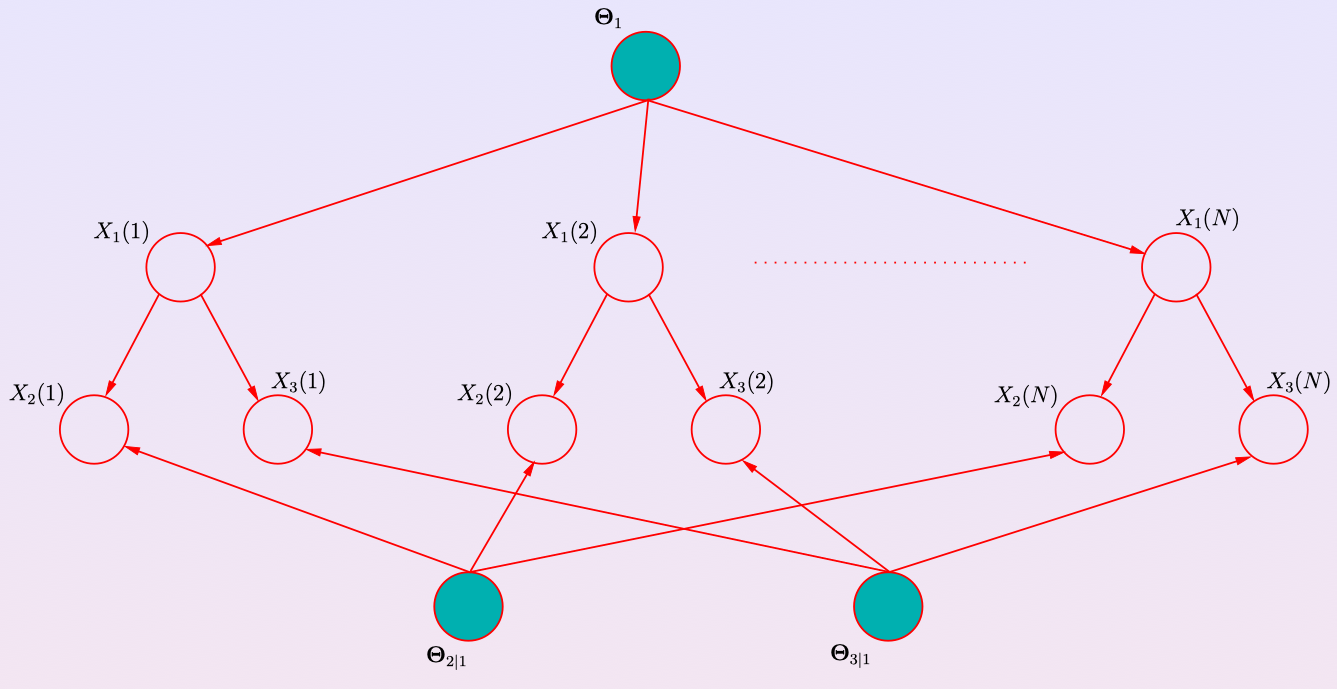
\includegraphics[width=0.6\linewidth]{LearningBN}
\end{center}
The parameters $\vect{\theta}$ of the network are the ones in blue, and they are connected to the nodes that depend on the parameters. Now we can compute the likelihood as follows since the examples are independent given $\vect{\theta}$:
\[P(\mathcal{D}\vert \vect{\theta})=\Prod_{i=1}^{N}P(\vect{x}(i)\vert\vect{\theta})\]
Then if we consider the factorization of the Bayesian Network we have
\[P(\mathcal{D}\vert\vect{\theta})=\Prod_{i=1}^N\Prod_{j=1}^mP(\vect{x}_j(i)\vert \text{pa}_j(i),\vect{\theta})\]
As it's possible to see from the previous graph, if, for instance, we'd want to compute the distribution of $\vect{\theta}_{3\vert 1}$, there is no reason for which we should also keep in consideration $x_2(2)$ since they are not connected:
\[P(\mathcal{D}\vect{\theta})=\Prod_{i=1}^N\Prod_{j=1}^mP(\vect{x}_j(i)\vert \text{pa}_j(i),\vect{\theta}_{X_j\vert\text{pa}_j}\]
Giving the disjoint conditional probability distribution. \newline
The parameters of CPD can be estimated independently, the estimate of the parameter $X_j$ by the maximum likelihood method is its maximum value:
\[\vect{\theta}^{\text{max}}_{X_j\vert\Pa{j}}=\argmax{\vect{\theta}_{X_j\vert \Pa{j}}}\Prod_{i=1}^NP(\vect{x}_j(i)\vert \Pa{j}(i),\vect{\theta}_{X_j\vert\Pa{j}})\]
The second part is nothing but the likelihood of the parameters and the dataset: 
\[\vect{\theta}^{\text{max}}_{X_j\vert\Pa{j}}=\argmax{\vect{\theta}_{X_j\vert \Pa{j}}}\Prod_{i=1}^NP(\vect{x}_j(i)\vert \Pa{j}(i),\vect{\theta}_{X_j\vert\Pa{j}})=\mathcal{L}(\vect{\theta}_{X_j\vert\Pa{j}},\mathcal{D})\]
A discrete CPD $P(X\vert \vect{U})$ can be represented as a table with:
\begin{itemize}
  \item A number of rows equal to the number $\Val{X}$ of configurations for $X$;
  \item A number of columns equal to the number $\Val{\vect{U}}$ of configurations for its parents $\vect{U}$;
  \item Each table entry $\theta_{x\vert\vect{u}}$ indicating the probability of a specific configuration $X=x$ and its parents $\vect{U}=\vect{u}$
\end{itemize}
Let's say we have this table sui fogli. allora possiamo massimizzare per ogni colonna quindi
\begin{center}
	%$\displaystyle argmax_{\theta_{T\vert T}, \theta_{F\vert T}}=\Pi_{i=x_2(i)=T}P(x_2(i)\vert x_2(i)=T, \theta_{T\vert T}, \theta_{F\vert T}$
\end{center}
E poi l'altra per l'altra colonna... \newline
Il numero di colonne è il prodotto di tutti i possibili padri per il numero di possibili valori che assume. Vedi quaderno 








